\documentclass[12pt]{nmsuth01}
%If your system does not have a latex package ``pkg'', for example,
 %attempting to run latex on the file will produce an error report
 %reading something like ``Latex error:  File pkg.sty not found.''
%
%Your system should have the latex symbol package.  If not comment out 
 %the next line by placing a percent sign % at the beginning of the line.
\usepackage{latexsym}
%Your system may not have the American Mathematical Society packages
 %for mathematics and theorem formatting.  If not, comment out the
 %next line.  If you comment out the next line, you should also
 %comment out all the theorem formatting commands, and you should not
 %try to process the part of the document called chp1a.tex.  Commment
 %out the line below calling for \input{chp1a}.
\usepackage{amsmath,amsthm}
%Your system may not have the xypic drawing package.  If not, comment
 %out the next line.  If you comment out the next line, you should
 %also not try to process chp1a.tex.  
\usepackage[all]{xy}
%Your system should have the graphicx package for included graphics.
 %If not, or, if you have no graphics to include, comment out the next 
 %line.  If you commment out the next line, then you should not try to 
 %process the part of the document called graphics.tex.  Comment out
 %the line below calling for \section{SAMPLE TEXT WITH GRAPHICS} \label{graphics}
%This file illustrates how include in your thesis graphical
 %output.
%The next line produces an indented paragraph to start the document
 %unit.  The LaTeX defaults start most units without indentations.
\hspace{\parindent}
This is sample text with graphics.
\begin{figure}[h]
  \centering
  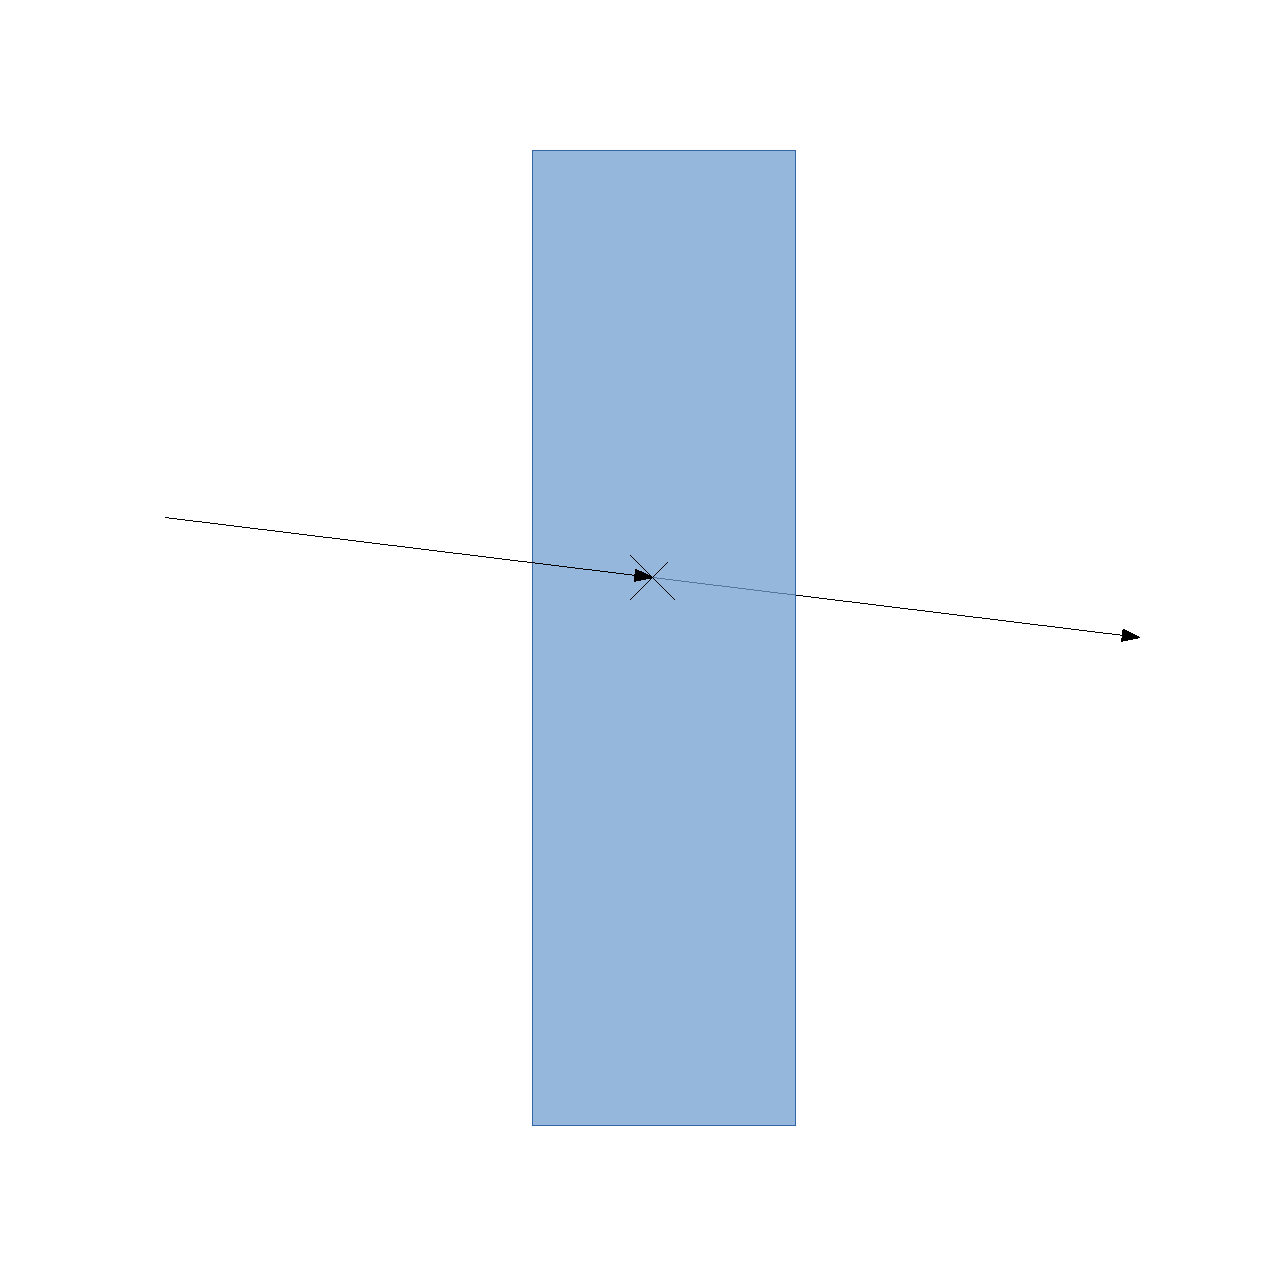
\includegraphics[angle=-90,width=4in]{figures/bz.pdf}
  \caption{This is an inserted EPS graphic}
  \label{fig:mygraph1}
\end{figure}
Sample ref of \ref{fig:mygraph1} 

\begin{figure}[t]
 \centering
  \includegraphics[angle=-90, width=4in]{figures/E734eta.pdf}  
    \caption{This is another inserted PDF graphic}
    \label{fig:mygraph2}
\end{figure}
%This is the end of the file graphics.tex


\usepackage{graphicx}
\usepackage{subcaption}
%The next settings give the correct margins for an NMSU Ph.D. thesis.
\setlength{\evensidemargin}{0.5in}
\setlength{\oddsidemargin}{0.5in}
\setlength{\textwidth}{5.75in}
\setlength{\topmargin}{-0.25in}
\setlength{\textheight}{8.25in}
%
%
% Theorem Formatting Commands.
\theoremstyle{plain}
\newtheorem{lemma}{Lemma}[section]
\newtheorem{prop}{Proposition}[section]
\newtheorem{theorem}{Theorem}[section]
\newtheorem{cor}{Corollary}[section]
%\newtheorem*{nametheorem}{Theorem}[section]
\theoremstyle{definition}
\newtheorem{defn}{Definition}[section]
\newtheorem{example}{Example}[section]
\theoremstyle{remark}
\newtheorem*{rem}{Remark}
\newtheorem*{convention*}{Convention}
%
% Miscellaneous Special Capitals
\newcommand{\bZ}{{\mathbf Z}}
\newcommand{\bQ}{{\mathbf Q}}
\newcommand{\bR}{{\mathbf R}}
\newcommand{\cC}{{\mathcal C}}
% 
%Miscellaneous symbols
\newcommand{\op}{{\rm \oplus}}
\newcommand{\id}{\rm id}
%
%Miscellaneous Greek letters
\newcommand{\eps}{\ensuremath{\epsilon}}
\newcommand{\ga}{\ensuremath{\gamma}}
%
%Miscellaneous operators
\DeclareMathOperator{\Coker}{Coker}
\DeclareMathOperator{\Tor}{Tor}
\DeclareMathOperator{\Ext}{Ext}
\DeclareMathOperator{\Maps}{Maps}
\DeclareMathOperator{\Hom}{Hom}
\DeclareMathOperator{\Aut}{Aut}
\DeclareMathOperator{\Sin}{Sin}
\DeclareMathOperator{\Tot}{Tot}
\DeclareMathOperator{\im}{im}
%
%Prepare for  double spacing
%\renewcommand{\baselinestretch}{1.5}
\newlength{\singlespace}
\setlength{\singlespace}{\baselineskip}
\newlength{\doublespace}
\setlength{\doublespace}{2.0\baselineskip}
%
\begin{document}
%Use the next line to obtain double spacing for the main body of the document
\setlength{\baselineskip}{\doublespace}
%Comment out the preceding line and uncomment the next line containing
 %a \setlength command to obtain single spacing for the main body of 
 %the document.
%\setlength{\baselineskip}{\singlespace}
%
%Why do you care about this option?
%There are two answers.  One is that it takes less paper to print a
 %preliminary draft of the thesis.  The second is that singlespacing
 %makes the structural units of the document more apparent.  Single
 %spacing makes it easy to identify definitions, lemmas, theorems, and 
 %so on, and it makes apparent such problems as a paragraph that is
 %running too long. On the other hand, the double spacing is good for 
 %checking for typographical errors in a manuscript.  Note that a 
 %document printed in singlespacing and doublespacing formats will 
 %have its problems with page and line breaks in different locations.  
%
%The title page, approval page, dedication page, acknowledgment page,
 %vita page, abstract page, and pages listing tables and figures (if
 %there are any) all carry roman numerals.
\pagenumbering{roman}
\pagestyle{empty}
%This file makes a title page for a Ph.D. thesis.
\thispagestyle{empty}
\renewcommand{\baselinestretch}{2}
\begin{center}
NEUTRAL CURRENT ELASTIC SCATTERING \\ AND THE STRANGE SPIN STRUCTURE OF THE PROTON
\vspace{0.1in}
BY\\
\vspace{0.1in}
KATHERINE WOODRUFF
\end{center}
\vspace{1.0in}
\begin{center}
A dissertation submitted to the Graduate School\\
\vspace{0.1in}
in partial fulfillment of the requirements\\
\vspace{0.1in}
for the degree \\
\vspace{0.1in}
Doctor of Philosophy
\end{center}
\vfill
\begin{center}
Major Subject: Physics
\end{center}
\vspace{1.0in}
\begin{center}
New Mexico State University\\
\vspace{0.1in}
Las Cruces New Mexico\\
\vspace{0.1in}
November 2018
\end{center}
\newpage
%This is the end of the title page.

\pagestyle{plain}
%This file makes the approval page for a Ph.D. thesis at NMSU.  It
 %must be replaced when a permanent Dean of the Graduate School is named.
\noindent
``Neutral Current Elastic Scattering and the Strange Spin Structure of the Proton,'' 
a dissertation prepared by
Katherine Woodruff 
in partial fulfillment of the requirements for the degree, 
Doctor of Philosophy,
has been approved and accepted by the following:

\setlength{\baselineskip}{\singlespace}
\vspace{0.1in}
\begin{flushleft}
\hrulefill
\newline
Dr. Luis Cifuentes
\newline
Dean of the Graduate School
\vspace{0.5in}

\hrulefill
\newline
Vassili Papavassiliou
\newline
Chair of the Examining Committee
\vspace{0.5in}

\hrulefill
\newline
Date
\vspace{0.5in}
\newline
Committee in charge:
\end{flushleft}

\setlength{\baselineskip}{\doublespace}
Dr. Vassili Papavassiliou, Chair

Dr. Stephen Pate

Dr. Igor Vasiliev

Dr. Steven Stochaj

\newpage
%This is the end of the approval page.

%
%This file makes a dedication page.
\begin{center}
DEDICATION
\end{center}
%The next blank line is needed to have the dedication text
 %appropriately indented.

I dedicate this work to my mom, dad, sister, bill.

\newpage
%This is the end of the dedication page.

%
%This file makes a page for acknowledgments.
\begin{center}
ACKNOWLEDGMENTS
\end{center}
%The next blank line is needed to have the dedication text
 %appropriately indented.

I would like to thank my advisor, ...

\newpage
%This is the end of the page for acknowledgments.

%
%This file makes a vita page in the required two column format.
\begin{center}
            VITA
\end{center}
\begin{flushleft}
\begin{tabular}{ll}
2006-2009        &  A.S., Linn-Benton Community College, Albany, Oregon
\\
& \\
2009-2012        &  B.S., University of Oregon, Eugene, Oregon
\\
& \\
2012-2015        &  M.S., New Mexico State University, Las Cruces, New Mexico
\end{tabular}
\end{flushleft}
\vspace{0.1in}
\begin{center}PUBLICATIONS
\end{center}
  C. Adams \textit{at al.}, "A Deep Neural Network for Pixel-Level Electromagnetic Particle Identification in the MicroBooNE Liquid Argon Time Projection Chamber”," \textit{Submitted to: Phys. Rev. D}, 2018. \\
  C. Adams \textit{at al.}, "Comparison of Muon-Neutrino-Argon Multiplicity Distributions Observed by MicroBooNE to GENIE Model Predictions," \textit{Submitted to: Phys. Rev. D}, 2018. \\
  C. Adams \textit{at al.}, "Ionization Electron Signal Processing in Single Phase LAr TPCs II: Data/Simulation Comparison and Performance in MicroBooNE," \textit{JINST}, vol. 13, no. 07, p. P07007, 2018. \\
  C. Adams \textit{at al.}, "Ionization Electron Signal Processing in Single Phase LAr TPCs I: Algorithm Description and Quantitative Evaluation with MicroBooNE Simulation," \textit{JINST}, vol. 13, no. 07, p. P07006, 2018. \\
  R. Acciarri \textit{at al.}, "The Pandora Multi-Algorithm Approach to Automated Pattern Recognition of Cosmic Ray Muon and Neutrino Events in the MicroBooNE Detector," \textit{Eur. Phys. J.}, vol. C78, p. 82, 2018. \\
  R. Acciarri \textit{at al.}, "Measurement of Cosmic Ray Reconstruction Efficiencies in the MicroBooNE LAr TPC Using a Small External Cosmic Ray Counter," \textit{JINST}, vol. 12, no. 12, p. P12030, 2017. \\
  R. Acciarri \textit{at al.}, "Noise Characterization and Filtering in the MicroBooNE Liquid Argon TPC," \textit{JINST}, vol. 12, no. 08, p. P08003, 2017. \\
  R. Acciarri \textit{at al.}, "Michel Electron Reconstruction Using Cosmic-Ray Data from the MicroBooNE LArTPC," \textit{JINST}, vol. 12, no. 09, p. P09014, 2017. \\
  P. Abratenko \textit{at al.}, "Determination of Muon Momentum in the MicroBooNE LArTPC Using an Improved Model of Multiple Coulomb Scattering," \textit{JINST}, vol. 12, no. 10, p. P10010, 2017. \\
  R. Acciarri \textit{at al.}, "Convolutional Neural Networks Applied to Neutrino Events in a Liquid Argon Time Projection Chamber," \textit{JINST}, vol. 12, no. 03, p. P03011, 2017. \\
   R. Acciarri \textit{et al.}, "Design and Construction of the MicroBooNE Detector," \textit{JINST}, vol. 12, no. 02, p. P02017, 2017. \\
\begin{center}
FIELD OF STUDY
\end{center}
\begin{flushleft}
Major Field: Experimental Particle Physics
\end{flushleft}

\newpage
%This is the end of the vita page.

%
%This file makes an abstract for a Ph.D. thesis.
\begin{center}
ABSTRACT
\end{center}
\vspace{0.3in}
\begin{center}
THESIS\\ TITLE
\\
BY
\\
KATHERINE WOODRUFF
\end{center}
\vspace{0.3in}
\begin{center}
Doctor of Philosophy

New Mexico State University

Las Cruces, New Mexico, 201?

Dr. Vassili Papavassiliou, Chair
\end{center}
\vspace{0.3in}
%The next line produces an indented paragraph to start the document
 %unit.  The LaTeX defaults start most units without indentations.
\hspace{\parindent}
This is the abstract.

\newpage
%This is the end of the abstract.

\tableofcontents
%If you have tables you will use the next three lines to create a list 
 %of tables following the table of contents page.  If you have no
 %tables in your document, then you comment out the next three lines
 %by placing a percent sign (%) at the beginning of each line.  You
 %may also delete the next three lines if they are not needed.
\newpage
\listoftables
\addcontentsline{toc}{section}{LIST OF TABLES}
%If you have figures you will use the next three lines to create a
 %list of figures following the table of contents page (and the list
 %of tables, if there is one).  If you have no list of figures, then
 %you comment out the next three lines by placing a percent sign (%)
 %at the beginning of the line.  You may also delete the next three
 %lines if they are not needed.
\newpage
\listoffigures
\addcontentsline{toc}{section}{LIST OF FIGURES}
%The next two lines are essentially the start of the main body of the
 %thesis.  You go to a new page, start numbering in arabic numerals,
 %and input the introduction. 
\newpage
\pagenumbering{arabic}
%
\section{Introduction} \label{sec:intro}
%The next line produces an indented paragraph to start the document
 %unit.  The LaTeX defaults start most units without indentations.
\hspace{\parindent}

%%%%%%%%%%%%%%%%%%%%%%%%%%%%%%%%%%%%%%%%%%%%%%%%%%%%%%%%%%%
% Standard Model
%%%%%%%%%%%%%%%%%%%%%%%%%%%%%%%%%%%%%%%%%%%%%%%%%%%%%%%%%%%
\subsection{The Standard Model}\label{sec:standardmodel}

Quarks, nucleons, neutrinos. Electromagnetic and weak forces.


%%%%%%%%%%%%%%%%%%%%%%%%%%%%%%%%%%%%%%%%%%%%%%%%%%%%%%%%%%%
% Spin Structure of Nucleons
%%%%%%%%%%%%%%%%%%%%%%%%%%%%%%%%%%%%%%%%%%%%%%%%%%%%%%%%%%%
\subsection{The Spin Structure of Nucleons} \label{sec:nuctheory}

  \subsubsection{Spin Structure Functions}
  In inclusive lepton-nucleon deep inelastic scattering (DIS), it is useful to
  parameterize the scattering cross section in terms of nucleon structure
  functions $F_1(x)$, $F_2(x)$, $g_1(x)$, and $g_2(x)$. In the QCD parton
  model~\cite{Feynman:1969wa}, $x$ is the fraction of the nucleon's momentum
  carried by the quarks, and $g_1$ and $g_2$, the spin structure functions,
  parameterize the polarized DIS cross section~\cite{Thomas:2001kw}.

  The $g_1$ spin structure function can be written as a combination of the spin
  contribution from each of the quark flavors~\cite{Bass:2007zzb},
  \begin{equation*}
    g_1(x) \frac{1}{2}\sum_q e_q^2 \Delta q(x) \,,
  \end{equation*}
  where $q$ is the quark flavor ($q = u,d,s$), $e_q$ is the electric charge of
  the quark, and $\Delta q$ is the contribution from the quark spin
  contribution to the nucleon spin,
  \begin{equation*}
    \Delta q(x) = \big(q^{\uparrow} + \bar{q}^{\uparrow}\big)(x) 
      - \big(q^{\downarrow} + \bar{q}^{\downarrow}\big)(x) \,.
  \end{equation*}
  Here $q^{\uparrow}(x)$ \big($q^{\downarrow}(x)$\big) is the probability of
  finding a quark with momentum fraction $x$ with its spin polarized in the
  (opposite) direction of the nucleon's spin, and $\bar{q}^{\uparrow}(x)$
  \big($\bar{q}^{\downarrow}(x)$\big) is the probability of finding an
  antiquark with momentum fraction $x$ with its spin polarized in the
  (opposite) direction of the nucleon's spin. Integrating over the quark spin
  structure gives the net quark spin contribution to the nucleon spin
  \begin{equation*}
    \Delta q = \int_0^1 \Big[\big(q^{\uparrow} + \bar{q}^{\uparrow}\big)(x)
      - \big(q^{\downarrow} + \bar{q}^{\downarrow}\big)(x) \Big] dx \,.
  \end{equation*}

  \subsubsection{The Ellis-Jaffe Sum Rule}

  The Ellis-Jaffe sum rule~\cite{Ellis:1973kp} relates the integral of the
  $g_1$ spin structure function to the axial charges~\cite{Thomas:2001kw},
  \begin{align*}
    g_A &= \Delta u - \Delta d \\
    g_A^{(8)} &= \Delta u + \Delta d - 2\Delta s \\
    g_A^{(0)} &= \Delta u + \Delta d + \Delta s \,.
  \end{align*}
  where $g_A$ is the isovector axial charge, $g_A^{(8)}$ is the $SU(3)$ octet
  axial charge, and $g_A^{(0)}$ is the flavor-singlet axial charge. For the
  proton, the integral of the $g_1$ spin structure function is
  \begin{align*}
    S_p &= \int_0^1 dx g_{1p}(x)  \\
        &= \int_0^1 dx \Big[\frac{4}{18}\Delta u(x) 
        + \frac{1}{18} \Delta d(x) + \frac{1}{18} \Delta s(x) \Big] \,, \\
        &= \frac{4}{18}\Delta u + \frac{1}{18}\Delta d + \frac{1}{18}\Delta s \,, \\
        &= \frac{g_A}{12} + \frac{g_A^{(8)}}{38} + \frac{g_A^{(0)}}{9} \,.
  \end{align*}
  The axial charges can be determined through experimental measurements.  The
  isovector axial charge, $g_A$, can be obtained in neutron
  $\beta$-decay~\cite{Dubbers:1991bh}. Assuming $SU(3)$ symmetry, $g_A^{(8)}$
  can be obtained though hyperon $\beta$-decay. If the net strange contribution
  to the nucleon spin is assumed to be negligible, the flavor-singlet charge is
  equal to the $SU(3)$ octet charge,
  \begin{equation*}
     \Delta s \sim 0 \Rightarrow g_A^{(0)} = g_A^{(8)} \,.
  \end{equation*}

  One of the first experiments to test the Ellis-Jaffe sum rule through
  inclusive DIS was the European Muon Collaboration (EMC) at CERN in
  1989~\cite{Ashman:1987hv,Ashman:1989ig}. The EMC scattered polarized muons
  off of a polarized proton target and detected the scattered muon in a forward
  muon spectrometer. Figure~\ref{fig:emcej} shows the EMC measurement of the
  integral of the $g_1$ spin structure function as a function of the lower
  bound on the integral, $x_m$, and the expected value of the integral at $x_m
  = 0$ from the Ellis-Jaffe sum rule. There is a significant discrepancy
  between the measured value and the value expected from theory. Assuming that
  the discrepancy comes from the assumption that $\Delta s = 0$, and not the
  $SU(3)$ symmetry assumption, the extracted non-zero value of $\Delta s$ to
  resolve the difference is
  \begin{equation*}
    \Delta s_{\textrm{EMC}} = -0.095 \pm 0.016 \pm 0.023 \,.
  \end{equation*}
  \begin{figure}[h]
    \centering
    \includegraphics[angle=0,width=5.5in]{figures/intro/strfunctions/EMC_Ellis-Jaffe.png}
    \caption{The integral of the $g_1(x)$ spin structure function measured by
      the EMC experiment~\cite{Ashman:1989ig}.}
    \label{fig:emcej}
  \end{figure}
  This implies not only that the overall spin polarization of the strange
  quarks and antiquarks in the nucleon sea is nonzero, but that they are
  polarized in the opposite direction of the proton.

  After the EMC result, many subsequent polarized target inclusive DIS
  experiments tested the Ellis-Jaffe sum rule over the next few decades.
  See~\cite{Aidala:2012mv}~and~\cite{Bass:2007zzb} for detailed reviews.
  Several inclusive DIS polarized target experiments were performed at
  SLAC~\cite{Baum:1983ha,Anthony:1996mw,Abe:1998wq} with a polarized electron
  beam, at CERN with the polarized muon beam by the Spin Muon Collaboration
  (SMC)~\cite{Adeva:1993km,Adeva:1998vv} and by
  COMPASS~\cite{Alexakhin:2006oza}, the polarized electron or positron HERA
  beam at DESY by the
  HERMES~\cite{Ackerstaff:1997ws,Ackerstaff:1999ey,Airapetian:2006vy}
  collaboration. A more recent measurements of the violation of the
  Ellis-Jaffe sum rule from polarized muon inclusive DIS off of a polarized
  target in the COMPASS experiment in 2007 gives~\cite{Alexakhin:2006oza}
  \begin{equation*}
    \Delta s_{\textrm{COMPASS}} = -0.08 \pm 0.01 \pm 0.02 \,,
  \end{equation*}
  and from the HERMES experiment in 2007 gives~\cite{Airapetian:2006vy}
  \begin{equation*}
    \Delta s_{\textrm{HERMES}} = -0.085 \pm 0.013 \pm 0.008 \pm 0.009 \,.
  \end{equation*}

  The nucleon spin structure can also be studied through semi-inclusive deep
  inelastic scattering (SIDIS). In SIDIS, in addition to detecting the
  scattered lepton, at least one of the final state pions or kaons is detected.
  If the detected hadron has a high enough energy fraction, it can be assumed
  that it contains the quark that was struck by the lepton~\cite{Bass:2007zzb}.
  A factor is included in the measured spin structure functions that describes
  the probability of a struck quark producing a pion or kaon with the measured
  energy fraction. This factor is called a fragmentation function, and it can
  be used to reconstruct individual quark flavor contributions to the nucleon
  spin. Several experiments has made measurements of the strange quark spin
  through SIDIS including COMPASS~\cite{Alekseev:2009ac,Alekseev:2010ub} at
  CERN and HERMES~\cite{Airapetian:2003ct,Airapetian:2004zf,Airapetian:2008qf}
  at DESY.  Measurements of the strange quark polarization in the nucleon
  through SIDIS tend to favor much smaller values of $\Delta s$ that are
  consistent with zero. While these results depend less on $SU(3)$ flavor
  symmetry than inclusive DIS results, they do depend strongly on the choice of
  fragmentation functions.
  
  \subsubsection{Theoretical Lattice QCD Calculations}


%%%%%%%%%%%%%%%%%%%%%%%%%%%%%%%%%%%%%%%%%%%%%%%%%%%%%%%%%%%
% Neutrinos as a Nucleon Probe
%%%%%%%%%%%%%%%%%%%%%%%%%%%%%%%%%%%%%%%%%%%%%%%%%%%%%%%%%%%

\subsection{Neutrino Measurements of the Strange Spin Structure}
\label{sec:neutrinos}
  Since neutrinos only interact via the weak force, neutrino-nucleon elastic
  scattering is sensitive to the weak currents and are great tools for
  measuring the axial form factor, $G_A(Q^2)$.
  See~\cite{Lyubushkin:2008pe}~and~\cite{Formaggio:2013kya} for detailed
  reviews of the many measurements of $G_A^s(Q^2)$ through charged current
  quasi-elastic (CCQE) scattering. Neutral current (NC) elastic
  neutrino-nucleon scattering ($\nu N \rightarrow \nu N$) specifically is
  sensitive to the NC form factor $G_A^{NC}(Q^2)$ which contains
  contributions from the up, down, and strange quarks to the spin structure
  of the nucleon ($G_A(Q^2)$ only contains contribution from the up and down
  quarks).

  At the limit where the negative four-momentum transfer squared, $Q^2$, goes
  to zero, the NC axial form factor becomes a combination of the net spin
  contribution from each of the quarks to the nucleon spin~\cite{Bass:2007zzb},
  \begin{equation*}
    G_A^{NC}(Q^2 = 0) = \frac{1}{2}(\Delta u - \Delta s - \Delta s)
  \end{equation*}

  The reconstructed four-momentum transfer is
  determined entirely from the nucleon kinetic energy using
  \begin{align*}
    Q^2_N &= -q^2 = -(\bf{p'}_N - \bf{p}_N)^2 \\
          &= -(E'_N - E_N)^2 + (\bar{p}'_N - \bar{p}_N)^2 \\
          &= 2 T_N M_N,
  \end{align*}
  where $\bf{p}$ is four-momentum, $E$ is energy, $\bar{p}$ is
  three-momentum, $M$ is mass, $T$ is kinetic energy determined by the length
  of the track, the $N$ subscript represents the nucleon in the
  neutrino-nucleon interaction, the prime represents the final state, and the
  nucleon momentum in the nucleus is assumed to be small compared to the
  final nucleon momentum. This means that the ability to measure the axial
  form factor at low $Q^2$ in NC elastic neutrino-nucleon scattering depends
  on the experimental nucleon energy threshold.

  Two previous neutrino experiments have performed a measurement of $\Delta
  s$ through neutral current elastic neutrino-nucleon scattering. The first
  was the E734 experiment~\cite{Ahrens:1986xe} at Brookhaven National Lab (BNL) in
  1987, and the second was the MiniBooNE experiment~\cite{Aguilar-Arevalo:2010cx} at
  Fermilab in 2010.

  \subsubsection{The BNL E734 Experiment}\label{sec:e734}
  The main target and detector of the E734 experiment was 170~tons and was
  made of a combination of liquid scintillator cells and proportional drift
  tubes (PDTs). The liquid scintillator composed 80\% of the target and was
  used for calorimetry and timing, while the PDTs were used for position
  information. Additionally, there was a electromagnetic shower counter and a
  muon spectrometer just downstream of the main detector. The full detector
  schematic is shown in Fig.~\ref{fig:e734detector}.
  \begin{figure}[h]
    \centering
    \includegraphics[angle=0,width=5.5in]{figures/intro/experiments/E734detector.pdf}
    \caption{Schematic of the BNL E734 detector~\cite{Ahrens:1986xe}.}
    \label{fig:e734detector}
  \end{figure}
  The E734 detector sat in a neutrino beam at BNL that could run in either
  neutrino of antineutrino mode with a mean energy of 1.3~GeV for neutrino
  and 1.2~GeV for antineutrinos.

  A simultaneous fit to the neutrino-proton and antineutrino-proton neutral
  current elastic cross sections in the negative four-momentum squared range
  between $Q^2 = 0.45$~GeV$^2$ and $Q^2 = 1.05$~GeV$^2$ was performed to
  extract the neutral current axial form factor.
  \begin{figure}[h]
    \centering
    \begin{subfigure}[t]{2.5in}
      \includegraphics[angle=0,width=2.5in]{figures/intro/experiments/E734flux.pdf}
      \caption{Measured neutrino-proton and antineutrino-proton cross sections.}
      \label{fig:e734xsec}
    \end{subfigure}
    \hspace{2pt}
    \begin{subfigure}[t]{2.5in}
      \includegraphics[angle=0,width=2.5in]{figures/intro/experiments/E734eta.pdf}
      \caption{Extracted neutral current axial form factor parameters.}
      \label{fig:e734eta}
    \end{subfigure}
    \caption{Results from the Brookhaven E734 measurement of the neutral
    current elastic cross section.}
    \label{fig:e734results}
  \end{figure}
  Figure~\ref{fig:e734xsec} shows the measured data and the cross section
  fits. Figure~\ref{fig:e734eta} shows the bounds on the axial mass $M_A$ and
  $\eta$ from the fit. In the parameter estimation, the NC axial form factor
  was assumed to have the form
  \begin{equation}\label{eq:axdipole}
    G_A^{NC}(Q^2) = \frac{1}{2}\frac{g_A}{(1+Q^2/M_A^2)^2}(1+\eta) \,,
  \end{equation}
  where $g_A$ is the weak coupling constant, $M_A$ is the axial mass, and
  $\eta$ is a factor that encodes the difference between the charged current
  axial form factor and the strange axial form factor. This form assumes that
  both parts of the form factor have the exact same shape. If the difference
  is only due to the net spin contribution of the strange quark, $\Delta s$,
  then $\Delta s = -\eta g_A$ which was found to be $-0.15 \pm 0.09$ in this
  analysis.

  A later analysis of the E734 NC elastic data was
  performed~\cite{Garvey:1992cg} in which the strange part of the electric
  and magnetic form factors was not assumed to be zero. Four fits to the
  neutrino-proton and antineutrino-proton cross section data were performed.
  In the first fit, only the axial mass was allowed to vary and the strange
  quark contribution to the electric, magnetic, and axial form factors were
  all held fixed at zero. In the second, the strange contribution to the
  electric and magnetic form factors were fixed at zero, but the axial mass
  and the strange axial form factor were allowed to vary. In the third fit,
  all three strange form factors and the axial mass were allowed to vary, and
  in the last fit, the strange form factors were all allowed to vary, but the
  axial mass was held to the world average at the time, $M_A =
  1.032\pm0.036$~GeV. The same form of the axial form factor in
  Eq.~\ref{eq:axdipole} was assumed and the strange electric and magnetic
  form factors were assumed to have the same shape as the charged current
  electric and magnetic form factors. The extracted value of $\Delta s$
  ranged from $\Delta s = -0.13 \pm 0.09$ in the second fit to $\Delta s =
  -0.21 \pm 0.10$ in the fourth fit.  Each of the extracted $\Delta s$ values
  is consistent with the original measurement and with a $\Delta s$ being
  negative.  Additionally, a strong correlation between $\Delta s$ and $M_A$
  was again observed. In the first fit with $\Delta s$ fixed at zero, a best
  fit to the data was found when $M_A = 1.086 \pm 0.015$~GeV which is very
  consistent with the original results in~\cite{Ahrens:1986xe} shown in
  Fig.~\ref{fig:e734eta}.

  An additional analysis of the E734 data considering ratios of neutral
  current elastic interactions to charged current elastic interactions was
  performed~\cite{Alberico:1998qw}. Specifically, they looked at the
  asymmetry
  \begin{equation*}
    \mathcal{A}_p(Q^2) = \frac{\Big(\frac{d\sigma}{dQ^2}\Big)_{\nu p \rightarrow \nu p} - \Big(\frac{d\sigma}{dQ^2}\Big)_{\bar{\nu} p \rightarrow \bar{\nu} p} }{\Big(\frac{d\sigma}{dQ^2}\Big)_{\nu n \rightarrow \mu^- p} - \Big(\frac{d\sigma}{dQ^2}\Big)_{\bar{\nu} p \rightarrow \mu^+ n}} \,.
  \end{equation*}
  This asymmetry has an enhancement in the strange axial and magnetic form
  factors. It was found that the experimental uncertainty was too large to
  determine $\Delta s$ and that a large factor of the uncertainty was due to
  the uncertainty on the axial mass. This analysis also assumed the dipole
  form of the axial form factor in Eq.~\ref{eq:axdipole}.

  \subsubsection{The MiniBooNE Experiment}\label{sec:miniboonence}
  The main target and detector of the MiniBooNE experiment was 800 tons of
  scintillator oil in a 12.2~m diameter spherical tank. Charged particles
  from the neutrino interactions in the mineral oil produced Cherenkov light
  which was collected by 1520 8-inch PMTs surrounding the oil. A schematic of
  the detector is shown in Fig.~\ref{fig:miniboonedetector}.
  \begin{figure}[h]
    \centering
    \includegraphics[angle=0,width=4in]{figures/intro/experiments/miniboone.png}
    \caption{Schematic of the MiniBooNE detector~\cite{Cheng:2012yy}.}
    \label{fig:miniboonedetector}
  \end{figure}
  MiniBooNE sat in the Booster Neutrino Beam (BNB) at Fermilab that can run
  in either neutrino or antineutrino mode with an average neutrino energy of
  $\sim$800~MeV~\cite{Aguilar-Arevalo:2008yp}.

  A $\Delta s$ fit to the ratio of the neutrino-proton to the
  neutrino-nucleon NC elastic cross section in the proton kinetic energy
  between $T = 350$~MeV and $T = 800$~MeV. This corresponds to a negative
  four-momentum transfer range of $Q^2 = 0.66$~GeV$^2$ to $Q^2 =
  1.5$~GeV$^2$. Figure~\ref{fig:miniboonedeltas} shows the measured ratio and
  the fits to the data.
  \begin{figure}[h]
    \centering
    \includegraphics[angle=0,width=4.5in]{figures/intro/experiments/miniboone_deltas.png}
    \caption{Ratio of the neutrino-proton NC elastic cross section to the
    neutrino-nucleon NC elastic cross section measured in
    MiniBooNE~\cite{Aguilar-Arevalo:2010cx}.}
    \label{fig:miniboonedeltas}
  \end{figure}
  In the analysis, the dipole shape in Eq.~\ref{eq:axdipole} was used for the
  axial form factor. When the value of the axial mass was held to $M_A =
  1.35$~GeV$^2$ a value of $\Delta s = 0.08 \pm 0.26$ was found, and when the
  axial mass was held to $M_A = 1.23$~GeV$^2$ a value of $\Delta s = 0.00 \pm
  0.30$. Both of these values are consistent with the E734 measurement and
  with zero.

  A later analysis of the MiniBooNE data was performed which included a
  two-body current contribution to the cross section~\cite{Golan:2013jtj}.
  The inclusion of the two-body current was done using the NuWro Monte Carlo
  neutrino event generator~\cite{Golan:2012wx}. The original MiniBooNE
  analysis used the NUANCE Monte Carlo neutrino event
  generator~\cite{Casper:2002sd}. A simultaneous extraction of $\Delta s$ and
  the axial mass from the assymetry $\mathcal{A}_p(Q^2)$ assuming the dipole
  form of the axial form factor in Eq.~\ref{eq:axdipole} and including
  two-body currents resulted in an axial mass value of $M_A =
  1.1^{+0.13}_{-0.15}$~GeV and $\Delta s = -0.4^{+0.5}_{-0.3}$. This result
  of $\Delta s$ is consistent with the original MiniBooNE result and with
  zero.

  Very recently, another re-analysis of the MiniBooNE result was performed
  using updated lattice QCD calculations of the strange electric and magnetic
  form factors and the measured MiniBooNE NC elastic nucleon cross section
  was performed~\cite{Sufian:2018qtw}. Notably, this analysis used
  z-expansion fit to the NC axial form factor (described in
  Sec.~\ref{sec:zexpansion}). A value of $\Delta s = -0.196\pm 0.127\pm
  0.041$ was found. The result was used to predict the BNL E734 NC elastic
  $\nu p$ and $\bar{\nu} p$ measurement and was found to be consistent. The
  NC elastic cross section calculated using the results are shown compared to
  MiniBooNE data in Fig.~\ref{fig:sufianuboone} and compared to E734 data in
  Fig.~\ref{fig:sufiane734}.
  \begin{figure}[h]
    \centering
    \begin{subfigure}[t]{2.5in}
      \includegraphics[angle=0,width=2.5in]{figures/intro/experiments/Sufian_MiniBooNE.png}
      \caption{Extracted NC elastic cross section compared to MiniBooNE data.}
      \label{fig:sufianuboone}
    \end{subfigure}
    \hspace{2pt}
    \begin{subfigure}[t]{2.5in}
      \includegraphics[angle=0,width=2.5in]{figures/intro/experiments/Sufian_BNL.png}
      \caption{Extracted NC elastic cross section compared to E734 data.}
      \label{fig:sufiane734}
    \end{subfigure}
    \caption{Neutral current elastic cross section results
    from~\cite{Sufian:2018qtw}}.
    \label{fig:sufiane734}
  \end{figure}

  \subsubsection{Global Fits of the Strange Axial Form Factor}


%This is the end of introduction

\newpage
\section{Neutrino-Nucleon interactions} \label{sec:theory}
%The next line produces an indented paragraph to start the document
 %unit.  The LaTeX defaults start most units without indentations.
\hspace{\parindent}
This section describes the mathematical foundation for the analysis. It gives a
derivation of the neutral current elastic neutrino-proton cross section, how
the cross section depends on the vector and axial form factors, and the
relationship of the neutral current form factors to the ones measured in
charged current scattering. The section ends with a discussion of the shape of
the form factors that are used in the analysis.

%%%%%%%%%%%%%%%%%%%%%%%%%%%%%%%%%%%%%%%%%%%%%%%%%%%%%%%%%%%
% Particle interactions
%%%%%%%%%%%%%%%%%%%%%%%%%%%%%%%%%%%%%%%%%%%%%%%%%%%%%%%%%%%
\subsection{Two-particle interactions}
  The differential cross section for two-fermion scattering, shown in
  Fig.~\ref{fig:feynmantwofermion}, is given by Fermi's Golden
  Rule~\cite{Aitchison:2004cs}
  \begin{equation}\label{eq:twobodyxsec}
    \sigma = \int \frac{(2\pi)^4 |\mathcal{M}|^2}{4 \sqrt{(p_1\cdot p_2)^2 - m_1^2m_2^2}}
      \cross d\Phi_2(p_1+p_2;p_1',p_2') \,,
  \end{equation}
  where $d\Phi_2(p_1+p_2;p_1',p_2')$ is an element of two-body phase space
  given by
  \begin{equation}\label{eq:twobodyphase}
      d\Phi_2(p_1+p_2;p_1',p_2') = \delta^4(p_1+p_2 - p_1'-p_2')
        \frac{d^3\mathbf{p}_1'}{(2\pi)^3 2E_1'}\frac{d^3\mathbf{p}_2'}{(2\pi)^3 2E_2'} \,,
  \end{equation}
  $p_1$ and $p_2$ are the incoming four-momenta of the fermions $f_1$ and
  $f_2$, respectively, $p_1'$ and $p_2'$ are the outgoing fermion momenta,
  $m_1$ and $m_2$ are the fermion masses, $E_1'$ and $E_2'$ are the outgoing
  fermion energies, and $\mathcal{M}$ is the scattering amplitude.
  Combining Eqns.~\ref{eq:twobodyxsec}~and~\ref{eq:twobodyphase} gives
  \begin{equation}\label{eq:genxsec}
       \sigma = \int \frac{|\mathcal{M}|^2}{64\pi^2}
        \frac{\delta^4(p_1+p_2-p_1'-p_2')}{E_1'E_2'\sqrt{(p_1\cdot p_2)^2 - m_1^2m_2^2}}
        \, d\mathbf{p}_1'd\mathbf{p}_2' \,.
  \end{equation}
  \begin{figure}[ht]
    \centering
    \includegraphics[angle=0,width=4in]{figures/theory/f1f2_feynman.pdf}
    \caption{Feynman diagram of two-fermion scattering.}
    \label{fig:feynmantwofermion}
  \end{figure}

  The scattering amplitude is given by the matrix element of the scattering
  matrix, $S$, between the final and initial states ($\mathcal{M} =
  \phys*{f}{S}{i}$).  The general form of $S$ is~\cite{Aitchison:2004cs}
  \begin{equation}
    S = \sum_{n=0}^{\infty} \frac{(-i)^n}{n!}\int\dots\int d^4x_1 \, d^4x_2 \dots d^4x_n\,
      T\{\hat{\mathcal{H}}'_I(x_1)\hat{\mathcal{H}}'_I(x_2)\dots\hat{\mathcal{H}}'_I(x_n)\} \,,
  \end{equation}
  where $\hat{\mathcal{H}}'_I(x_i)$ is the interaction Hamiltonian density.
  
  The matrix element can more easily be determined using Feynman calculus.  For
  a massive, vector-boson propagator the matrix element for this interaction is
  given by~\cite{Aitchison:2004cs}
  \begin{equation}\label{eq:genmatel}
    \mathcal{M} = \phys*{f}{S}{i} = \phys*{p_1'}{J^{\mu}(0)}{p_1} \frac{i}{q^2 - M_V^2}(-g_{\mu\nu} 
            + q_{\mu}q_{\nu}/M_V^2) \phys*{p_2'}{J^{\mu}(0)}{p_2} \,,
  \end{equation}
  where $q$ is the four-momentum carried by the vector-boson propagator, $M_V$
  is the mass of the propagator, $J^{\mu}(0)$ is the probability current
  operator, and $g_{\mu\nu}$ is the metric tensor.


%%%%%%%%%%%%%%%%%%%%%%%%%%%%%%%%%%%%%%%%%%%%%%%%%%%%%%%%%%%
% Electroweak Interactions
%%%%%%%%%%%%%%%%%%%%%%%%%%%%%%%%%%%%%%%%%%%%%%%%%%%%%%%%%%%
\subsection{Electroweak interactions}

  The charged current, $j^{\mu}_{CC}$, which corresponds to the exchange of a
  $W^{\pm}$ boson, and the neutral current, $j^{\mu}_{NC}$, which corresponds
  to the exchange of the $Z^0$ boson are given by~\cite{Paschos:2007pi}
  \begin{align}\label{eq:ccurrent}
      j^{\mu}_{CC} &= \sum_f \bar{\psi}_f \gamma^{\mu} (1-\gamma_5) \frac{1}{2}(\tau_1 + i\tau_2) \psi_f \\
        \label{eq:ncurrent}
      j^{\mu}_{NC} &= \sum_f \bar{\psi}_f \gamma^{\mu} (1-\gamma_5) \frac{1}{2}(\tau_3) \psi_f 
       - 2\sin^2(\theta_W) j^{\mu}_{em}
  \end{align}
  where $j^{\mu}_{em}$ is the electromagnetic current, $\psi_{f}$ are the weak
  isospin doublets, and $\tau_i$ are the Pauli matrices
  \begin{equation}
      \tau_1 = 
      \begin{pmatrix}
        0 & 1 \\
        1 & 0
      \end{pmatrix} \,,
      \hspace{5mm}
      \tau_2 = 
      \begin{pmatrix}
        0 & -i \\
        i & 0
      \end{pmatrix} \,,
      \hspace{5mm}
      \tau_3 = 
      \begin{pmatrix}
        1 & 0 \\
        0 & -1
      \end{pmatrix} \,.
  \end{equation}
  The lepton weak isospin doublets are~\cite{Paschos:2007pi}
  \begin{equation}
    \psi_{e} = 
    \begin{pmatrix}
        \hat{\nu}_{e} \\
        \hat{e}^-
    \end{pmatrix} \,,
      \hspace{5mm}
    \psi_{\mu} = 
    \begin{pmatrix}
        \hat{\nu}_{\mu} \\
        \hat{\mu}^-
    \end{pmatrix} \,,
      \hspace{5mm}
    \psi_{\tau} = 
    \begin{pmatrix}
        \hat{\nu}_{\tau} \\
        \hat{\tau}^-
    \end{pmatrix} \,,
  \end{equation}
  and the quark weak isospin doublets are
  \begin{equation}
    \psi_{1} = 
    \begin{pmatrix}
        \hat{u} \\
        \hat{d'}
    \end{pmatrix} \,,
      \hspace{5mm}
    \psi_{2} = 
    \begin{pmatrix}
        \hat{c} \\
        \hat{s'}
    \end{pmatrix} \,,
      \hspace{5mm}
    \psi_{3} = 
    \begin{pmatrix}
        \hat{t} \\
        \hat{b'}
    \end{pmatrix} \,,
  \end{equation}
  where $d'$, $s'$, and $b'$ represent the ``mixed" states
  \begin{equation}
      \begin{pmatrix}
        \hat{d}' \\
        \hat{s}' \\
        \hat{b}'
      \end{pmatrix}
      =
      \begin{pmatrix}
          V_{ud} & V_{us} & V_{ub} \\
          V_{cd} & V_{cs} & V_{cb} \\
          V_{td} & V_{ts} & V_{tb}
      \end{pmatrix}
      \begin{pmatrix}
        \hat{d} \\
        \hat{s} \\
        \hat{b}
      \end{pmatrix} \,.
  \end{equation}
  The matrix, $V$, is the Cabibbo-Kobayashi-Maskawa matrix. These doublets
  contain the allowed weak transitions where $V_{ab}$ is the probability of a
  transition from a quark with flavor $a$ to a quark with flavor $b$.

  \subsubsection{The charged and neutral currents}
  The linear combination of Pauli matrices in the charged current
  \begin{equation}
      \frac{1}{2}\tau^+ = \frac{1}{2}(\tau_1 + \tau_2) \,,
  \end{equation}
  acts as an ``isospin raising matrix" and corresponds to the exchange of a
  $W^+$ boson.
  For the leptons, this gives~\cite{Paschos:2007pi}
  \begin{equation}
    \begin{aligned}
      j^{\mu}_{CC}(\textrm{leptons}) &= \sum_{l=e,\mu,\tau}
      \begin{pmatrix}
          \bar{\hat{\nu}}_l \\
          \bar{\hat{l}}
      \end{pmatrix}
      \gamma^{\mu}(1-\gamma_5)\frac{1}{2}
      \begin{pmatrix}
        0 & 1 \\
        0 & 0
      \end{pmatrix}
      \begin{pmatrix}
        \hat{\nu}_l \\
          \hat{l}
      \end{pmatrix} \\
      &= \sum_{l=e,\mu,\tau} \bar{\hat{\nu}}_{l} \gamma^{\mu}(1-\gamma_5)\frac{1}{2}\, \hat{l} \,,
    \end{aligned}
  \end{equation}
  and, similarly, for the quarks we get
  \begin{equation}
      j^{\mu}_{CC}(\textrm{quarks}) =
       \bar{\hat{u}}\gamma^{\mu}(1-\gamma_5)\frac{1}{2}\,\hat{d}'
       +\bar{\hat{c}}\gamma^{\mu}(1-\gamma_5)\frac{1}{2}\,\hat{s}'
       +\bar{\hat{t}}\gamma^{\mu}(1-\gamma_5)\frac{1}{2}\,\hat{b}' \,,
  \end{equation}
  with the total charged current being $j^{\mu}_{CC} =
  j^{\mu}_{CC}(\textrm{leptons}) + j^{\mu}_{CC}(\textrm{quarks})$.

  In neutral current scattering, $\frac{1}{2}\tau_3$ gives the weak isospin
  which acts as a ``weak charge". The electromagnetic current is given by
  \begin{equation}
      j^{\mu}_{em} = \sum_f Q_f \bar{\hat{f}} \gamma^{\mu} \hat{f}
  \end{equation}
  where the sum is over the fermion flavors, and $Q_f$ is the electric charge
  of $f$.  So, the total neutral current is
  \begin{equation}
    \begin{aligned}
        j^{\mu}_{NC} &= \sum_{l=e,\mu,\tau} \left(\bar{\hat{\nu}}_{l}
        \gamma^{\mu}(1-\gamma_5) \frac{1}{2}\, \hat{\nu}_{l} - \bar{\hat{l}}
        \gamma^{\mu}(1-\gamma_5) \frac{1}{2}\, \hat{l} 
        +\sin^2\theta_W \bar{\hat{l}}\gamma^{\mu}\hat{l} \right) \\
        &+ \sum_{q=u,c,t} \left(\bar{\hat{q}} \gamma^{\mu}(1-\gamma_5)\frac{1}{2}\hat{q} 
        - \sin^2\theta_W \frac{2}{3} \bar{\hat{q}}\gamma^{\mu}\hat{q} \right) \\
        &+ \sum_{q=d,s,b} \left(- \bar{\hat{q}} \gamma^{\mu}(1-\gamma_5)\frac{1}{2}\hat{q} 
        + \sin^2\theta_W \frac{1}{3} \bar{\hat{q}}\gamma^{\mu}\hat{q} \right) \,.
     \end{aligned}
  \end{equation}
 
  \subsubsection{V$-$A structure}

  We can separate the currents into their vector and pseudovector, or axial
  vector, components. The terms that contain just $\gamma^{\mu}$ behave like
  vectors under a parity transformation~\cite{Alberico:2001sd}
  \begin{equation}
    \hat{\textrm{\textbf{P}}}\hat{\psi}(\textbf{x},t)\hat{\textrm{\textbf{P}}}^{-1} \, 
      \gamma^{\mu} \, \hat{\textrm{\textbf{P}}}\hat{\psi(\textbf{x},t)}\hat{\textrm{\textbf{P}}}^{-1} 
      = - \hat{\textrm{\textbf{P}}}\hat{\psi}(-\textbf{x},t)\hat{\textrm{\textbf{P}}}^{-1} \, 
      \gamma^{\mu} \, \hat{\textrm{\textbf{P}}}\hat{\psi(-\textbf{x},t)}\hat{\textrm{\textbf{P}}}^{-1}
  \end{equation}
  where $\hat{\textrm{\textbf{P}}}$ is the parity operator
  \begin{equation}
    \textrm{\textbf{P}}: \textbf{x} \rightarrow -\textbf{x}, t \rightarrow t \,.
  \end{equation}
  The terms that contain $\gamma^{\mu}\gamma_{5}$ behave like axial vectors
  under a parity transformation
  \begin{equation}
    \hat{\textrm{\textbf{P}}}\hat{\psi}(\textbf{x},t)\hat{\textrm{\textbf{P}}}^{-1} \, 
      \gamma^{\mu}\gamma_5 \, \hat{\textrm{\textbf{P}}}\hat{\psi(\textbf{x},t)}\hat{\textrm{\textbf{P}}}^{-1} 
      = + \hat{\textrm{\textbf{P}}}\hat{\psi}(-\textbf{x},t)\hat{\textrm{\textbf{P}}}^{-1} \, 
      \gamma^{\mu}\gamma_5 \, \hat{\textrm{\textbf{P}}}\hat{\psi(-\textbf{x},t)}\hat{\textrm{\textbf{P}}}^{-1}
      \,.
  \end{equation}
  The charged current is
  \begin{equation}
    \begin{aligned}
    j^{\mu}_{CC} = \frac{g}{\sqrt{2}}\Bigg[&\sum_{l=e,\mu,\tau} \bar{\hat{\nu}}_l (\gamma^{\mu} 
          - \gamma^{\mu}\gamma_5)\frac{1}{2}\,\hat{l} \\
      &+ \bar{\hat{u}}(\gamma^{\mu} - \gamma^{\mu}\gamma_5)\frac{1}{2}\, \hat{d}'
      + \bar{\hat{c}}(\gamma^{\mu} - \gamma^{\mu}\gamma_5)\frac{1}{2}\, \hat{s}'
      + \bar{\hat{t}}(\gamma^{\mu} - \gamma^{\mu}\gamma_5)\frac{1}{2}\, \hat{b}' \Bigg] \,,
    \end{aligned}
  \end{equation}
  and the neutral current becomes
  \begin{equation}
    \begin{aligned}
        j^{\mu}_{NC} = \frac{g}{2\cos\theta_W} \Bigg[&\sum_{l=e,\mu,\tau} 
        \left(\bar{\hat{\nu}}_{l}(g_V^{l} \gamma^{\mu}- g_A^{l} \gamma^{\mu}\gamma_5) \hat{\nu}_{l} 
         + \bar{\hat{l}}(g_V^{l} \gamma^{\mu}- g_A^{l} \gamma^{\mu}\gamma_5)\, \hat{l} \right) \\
        &+ \sum_{q=u,d,c,s,t,b} 
         \left(- \bar{\hat{q}} (g_V^{q} \gamma^{\mu}-g_A^{q} \gamma^{\mu}\gamma_5)\hat{q} \right)\Bigg] \,.
     \end{aligned}
  \end{equation}
  where 
  \begin{equation}
    g_V^{f} = \frac{1}{2}\tau_3^{f} - 2\sin^2\theta_W Q_f \,,
    \hspace{3mm}
    g_A^{f} = \frac{1}{2}\tau_3^{f} \,.
  \end{equation}

%%%%%%%%%%%%%%%%%%%%%%%%%%%%%%%%%%%%%%%%%%%%%%%%%%%%%%%%%%%
% Electroweak Scattering Matrix Elements
%%%%%%%%%%%%%%%%%%%%%%%%%%%%%%%%%%%%%%%%%%%%%%%%%%%%%%%%%%%
\subsection{Electroweak Scattering Matrix Elements}

  \begin{figure}[h]
    \centering
    \begin{subfigure}{2.5in}
      \includegraphics[angle=0,width=2.5in]{figures/theory/nun_feynman.pdf}
      \caption{Feynman diagram of charged-current elastic lepton-nucleon
      scattering.}
      \label{fig:ccqefeynman}
    \end{subfigure}
    \hspace{2pt}
    \begin{subfigure}{2.5in}
      \includegraphics[angle=0,width=2.5in]{figures/theory/nup_feynman.pdf}
      \caption{Feynman diagram of neutral-current elastic lepton-nucleon
      scattering.}
      \label{fig:ncefeynman}
    \end{subfigure}
  \end{figure}

  To calculate the charged-current neutrino-nucleon scattering matrix element,
  as shown in Fig.~\ref{fig:ccqefeynman}, we need to determine the lepton CC
  matrix element, $_{l}{\phys*{k'}{J^{\mu}_{CC}(0)}{k}}_{\nu_l}$, and the nucleon
  CC matrix element, $_{\textrm{p}}{\phys*{p'}{J^{\mu}_{CC}(0)}{p}}_{\textrm{n}}$,
  and for neutral-current, as shown in Fig.~\ref{fig:ncefeynman}, we need the
  lepton NC matrix element, $_{\nu_l}\phys*{k'}{J^{\mu}_{NC}(0)}{k}_{\nu_l}$, and
  the nucleon NC matrix element,
  $_{\textrm{p}}\phys*{p'}{J^{\mu}_{NC}(0)}{p}_{\textrm{p}}$. Leptons are
  point-like particles, so their matrix elements are straight-forward
  \begin{equation}\label{eq:leptonmatel}
    \begin{aligned}
      _l\phys*{k'}{J^{\mu}_{CC}(0)}{k}_{\nu_l}
        &= -i\frac{G_F}{\sqrt{2}}\bar{u}(k')(\gamma^{\mu} - \gamma^{\mu}\gamma_5)u(k) \,, \\
        _{\nu_l}\phys*{k'}{J^{\mu}_{NC}(0)}{k}_{\nu_l}
        &= -\frac{G_F}{\sqrt{2}}\bar{u}(k')(\gamma^{\mu} - \gamma^{\mu}\gamma_5)u(k) \,.
    \end{aligned}
  \end{equation}

  \subsubsection{Nucleon matrix elements}
  Since nucleons have a finite structure, the nucleon matrix elements have a
  more complicated form. The current is corrected by form factors which encode
  the longitudinal nucleon structure.

  If we define the vector and axial parts of the nucleon currents by
  \begin{equation}
    \begin{aligned}
    v^{\mu}_i &= \bar{\hat{\psi}}_f\, \gamma^{\mu}\frac{1}{2}\tau_i\, \hat{\psi}_f \,, \\
    a^{\mu}_i &= \bar{\hat{\psi}}_f\, \gamma^{\mu}\gamma_5\frac{1}{2}\tau_i\, \hat{\psi}_f \,,
    \end{aligned}
  \end{equation}
  where $\hat{\psi}$ are the quark doublets and $\tau_i$ are the Pauli matrices
  still, then the nucleon charged and neutral current become
  \begin{equation}
    \begin{aligned}
      j^{\mu}_{CC} &= v^{\mu}_+ - a^{\mu}_+ \,, \\
      j^{\mu}_{NC} &= v^{\mu}_3 - a^{\mu}_3 - 2\sin^2\theta_W j^{\mu}_{em;q} \,,
    \end{aligned}
  \end{equation}
  where $v^{\mu}_+ = v^{\mu}_1 + iv^{\mu}_2$ and $a^{\mu}_+ = a^{\mu}_1 +
  ia^{\mu}_2$. The nucleon matrix elements become
  \begin{equation}
    \begin{aligned}
      _{\textrm{p}}\phys*{p'}{J^{\mu}_{CC}}{p}_{\textrm{n}}
          &= \prescript{}{\textrm{p}}{\phys*{p'}{V^{\mu}_{+}}{p}}_{\textrm{n}}
            - \prescript{}{\textrm{p}}{\phys*{p'}{A^{\mu}_{+}}{p}}_{\textrm{n}} \,, \\
      _{\textrm{p}}\phys*{p'}{J^{\mu}_{NC}}{p}_{\textrm{p}}
          &= \prescript{}{\textrm{p}}{\phys*{p'}{V^{\mu}_{3}}{p}}_{\textrm{p}} 
            - \prescript{}{\textrm{p}}{\phys*{p'}{A^{\mu}_{3}}{p}}_{\textrm{p}} 
            - \prescript{}{\textrm{p}}{\phys*{p'}{J^{\mu}_{em}}{p}}_{\textrm{p}} \,,
    \end{aligned}
  \end{equation}
  where $J^{\mu}$, $V^{\mu}$, and $A^{\mu}$ are current operators.

  \subsubsection{Electromagnetic Scattering}

  It is easiest to first find an equation for $j^{\mu}_{em;q}$ in terms of the
  electric and magnetic form factors. The nucleon electromagnetic current
  should have the same vector form as the electromagnetic current for
  point-like particles. The available physical variables to construct the
  nucleon EM current are $p$, $p'$, $\gamma^{\mu}$. The most general form
  is~\cite{Alberico:2001sd}
  \begin{equation}
    \Gamma^{\mu} = \gamma^{\mu}\cdot A + (p'^{\mu} + p^{\mu})\cdot B + (p'^{\mu} - p^{\mu})\cdot C \,,
  \end{equation}
  where $\Gamma^{\mu}$ is given by the equation
  $_{\textrm{p}}\phys*{p'}{J^{\mu}_{em}(0)}{p}_{\textrm{p}} =
  \bar{u}(p')\Gamma^{\mu}u(p)$, and $A$, $B$, and $C$ are arbitrary form
  factors.  $\Gamma^{\mu}$ is constrained further by the Ward
  identity~\cite{Ward:1950xp}, $q_{\mu}\Gamma^{\mu} = 0$, which guarantees
  current conservation. The $\gamma^{\mu}$ and $(p'^{\mu} + p^{\mu})$ terms in
  $q_{\mu}\Gamma^{\mu}$ go to zero, but the $(p'^{\mu} - p^{\mu})$ term does
  not, so $C=0$. Using the Gordon identity~\cite{Gordon:1928}, the general form
  for the nucleon EM current matrix element is
  \begin{equation}\label{eq:FFem}
    _{\textrm{p}}\phys*{p'}{J^{\mu}_{em}(0)}{p}_{\textrm{p}} =
      \bar{u}(p')\left[ \gamma^{\mu}F_1(Q^2) + \frac{i\sigma^{\mu\nu}q_{\mu}}{2M}F_2(Q^2)  \right]u(p) \,.
  \end{equation}
  The form factors $F_1$ and $F_2$ are the Dirac and Pauli form factors,
  respectively, and they are functions of $Q^2 = -q^2$, the negative
  four-momentum transfer. They can be transformed into the Sachs form factors,
  $G_E$ and $G_M$ by the relationships
  \begin{equation}
    G_E(Q^2) = F_1(Q^2) - \frac{Q^2}{4M^2}F_2(Q^2)\,, \hspace{5mm} G_M(Q^2) = F_1(Q^2) + F_2(Q^2) \,.
  \end{equation}
  The electric form factor, $G_E$ encodes the longitudinal electric charge
  structure of the nucleon and the magnetic form factor, $G_M$, encodes the
  longitudinal magnetic structure. At the limit when $Q^2$ goes to zero, the
  Sachs form factors become the net charge and magnetic moment of the nucleon.
  \begin{equation}
    \begin{aligned}
      G_{E;p}(Q^2=0) = 1 \,,& \hspace{5mm} G_{M;p}(Q^2=0) = \mu_p \,, \\
      G_{E;n}(Q^2=0) = 0 \,,& \hspace{5mm} G_{M;n}(Q^2=0) = \mu_n \,,
    \end{aligned}
  \end{equation}
  where $\mu_p$ and $\mu_n$ are the proton and neutron magnetic moments.
 
  \subsubsection{Vector current}

    The quark part of the electromagnetic current, $j^{\mu}_{em;q}$, can be
    written as~\cite{Alberico:2001sd}
    \begin{equation}\label{eq:emcurrent30}
      \begin{aligned}
        j^{\mu}_{em;q} &= \bar{\hat{\psi}}_f \, Q_f \gamma^{\mu}\, \hat{\psi}_f \\
                       &= \bar{\hat{\psi}}_f \, (\tau_3 + \frac{1}{6})\gamma^{\mu} \, \hat{\psi}_f \\
                       &= v^{\mu}_3 + v^{\mu}_0 \,,
      \end{aligned}
    \end{equation}
    where $v^{\mu}_0 = \frac{1}{6}\bar{\hat{\psi}}_f \, \gamma^{\mu}
    \hat{\psi}_f$. Now we can write the nucleon electromagnetic current matrix
    element in terms of the vector and isoscalar parts
    \begin{equation}
      \begin{aligned}
        _{\textrm{p(n)}}\phys*{p'}{J^{\mu}_{em}(0)}{p}_{\textrm{p(n)}} 
            &= \prescript{}{\textrm{p(n)}}{\phys*{p'}{V^{\mu}_3(0) + V^{\mu}_0(0))}{p}}_{\textrm{p(n)}} \\
            &= \prescript{}{\textrm{p(n)}}{\phys*{p'}{V^{\mu}_3(0)}{p}}_{\textrm{p(n)}} 
             + \prescript{}{\textrm{p(n)}}{\phys*{p'}{V^{\mu}_0(0)}{p}}_{\textrm{p(n)}} \,,
      \end{aligned}
    \end{equation}
    Since $V^{\mu}_3$ behaves as a vector under the charge symmetry operator
    and $V^{\mu}_0$ behaves as a scalar, the following equations are true
    \begin{equation}
      \begin{aligned}
        \prescript{}{\textrm{p}}{\phys*{p'}{V^{\mu}_3(0)}{p}}_{\textrm{p}} 
          &= - \prescript{}{\textrm{n}}{\phys*{p'}{V^{\mu}_3(0)}{p}}_{\textrm{n}} \,, \\
        \prescript{}{\textrm{p}}{\phys*{p'}{V^{\mu}_0(0)}{p}}_{\textrm{p}} 
          &= + \prescript{}{\textrm{n}}{\phys*{p'}{V^{\mu}_0(0)}{p}}_{\textrm{n}} \,. \\
      \end{aligned}
    \end{equation}
    Then
    \begin{align}\label{eq:V3em}
      \prescript{}{\textrm{p}}{\phys*{p'}{V^{\mu}_3(0)}{p}}_{\textrm{p}} 
        &= \frac{1}{2} \left[\prescript{}{\textrm{p}}{\phys*{p'}{J^{\mu}_{em}(0)}{p}}_{\textrm{p}} 
         - \prescript{}{\textrm{n}}{\phys*{p'}{J^{\mu}_{em}(0)}{p}}_{\textrm{n}} \right] \,, \\
      \prescript{}{\textrm{p}}{\phys*{p'}{V^{\mu}_0(0)}{p}}_{\textrm{p}} 
        &= \frac{1}{2} \left[\prescript{}{\textrm{p}}{\phys*{p'}{J^{\mu}_{em}(0)}{p}}_{\textrm{p}} 
         + \prescript{}{\textrm{n}}{\phys*{p'}{J^{\mu}_{em}(0)}{p}}_{\textrm{n}} \right] \,.
    \end{align}
    Combining equations~\ref{eq:FFem}~and~\ref{eq:V3em} gives
    \begin{equation}
      \prescript{}{\textrm{p}}{\phys*{p'}{V^{\mu}_3(0)}{p}}_{\textrm{p}} 
        = \bar{u}(p') \left[\gamma^{\mu}F_1^V(Q^2) 
          + \frac{i\sigma^{\mu\nu}q_{\mu}}{2M}F_2^V(Q^2)\right] u(p) \,,
    \end{equation}
    where the vector form factors, $F_1^V$ and $F_2^V$ are defined as
    \begin{equation}
      \begin{aligned}
        F_1^V(Q^2) &= \frac{1}{2}\left( F_{1,\textrm{p}}(Q^2) - F_{1,\textrm{n}}(Q^2)\right) \,, \\
        F_2^V(Q^2) &= \frac{1}{2}\left( F_{2,\textrm{p}}(Q^2) - F_{2,\textrm{n}}(Q^2)\right) \,.
      \end{aligned}
    \end{equation}

    The isoscalar nucleon matrix element is then
    \begin{equation}
      {\phys*{p'}{V^{\mu}_0(0)}{p}}
      = \bar{u}(p')\left[\gamma^{\mu}\frac{1}{2}\left(F_{1,p}(Q^2) + F_{1,n}(Q^2)\right) 
        + \frac{i\sigma^{\mu\nu}q_{\mu}}{2M}\frac{1}{2}\left(F_{2,p}(Q^2) + F_{2,n}(Q^2)\right)\right]u(p)
    \end{equation}
 
    Under the conserved vector current (CVC)
  hypothesis~\cite{Gerstein:1956,Feynman:1958ty} the ``raising" and ``lowering"
  vector currents, $v^{\mu}_{\pm}$, in the charged current interactions are the
  same as the vector part of the electromagnetic current, $v^{\mu}_{3}$.

  \subsubsection{Axial current}

    The axial current nucleon matrix elements can also be parameterized in
    terms of form factors. Starting with the charged axial current, the most
    general form contains an axial, a pseudoscalar, and a tensor
    term,~\cite{Alberico:2001sd}
    \begin{equation}
      \prescript{}{\textrm{p}}{\phys*{p'}{A^{\mu}_+(0)}{p}}_{\textrm{n}} 
        = \bar{u}(p') \left[\gamma^{\mu}\gamma^{5} G_A(Q^2) 
          + \frac{q^{\mu}\gamma^{5}}{2M}G_P^{CC}(Q^2) 
          + \frac{i\sigma^{\mu\nu}q_{\mu}\gamma^{5}}{2M}G_T^{CC}(Q^2)\right] u(p) \,,
    \end{equation}
    where $G_A$, $G_P^{CC}$, and $G_T^{CC}$ are the axial form factors.  From
    isospin symmetry, we have
    \begin{equation}
      \prescript{}{\textrm{p}}{\phys*{p'}{A^{\mu}_+(0)}{p}}_{\textrm{n}} 
      = \prescript{}{\textrm{n}}{\phys*{p'}{A^{\mu}_-(0)}{p}}_{\textrm{p}} 
      \equiv \prescript{}{\textrm{p}}{\phys*{p}{A^{\mu}_+(0)}{p'}}_{\textrm{n}}^* \,,
    \end{equation}
    which implies that $G_T^{CC}(Q^2) = 0$. In quasi-elastic scattering the
    pseudoscalar term containing $G_P^{CC}(Q^2)$ is proportional to the lepton
    mass and can be ignored in neutral current scattering since $m_{\nu}\approx
    0$. The charged current axial matrix element is then just
    \begin{equation}
      \prescript{}{\textrm{p}}{\phys*{p'}{A^{\mu}_+(0)}{p}}_{\textrm{n}} 
        = \bar{u}(p') \,\gamma^{\mu}\gamma^{5} G_A(Q^2)\, u(p) \,.
    \end{equation}
    The form factor $G_A$ encodes the longitudinal spin structure of the
    nucleon due to the spin of the up and down quarks and is referred to as the
    charged current axial form factor, or just the axial form factor.

    The most general form for the neutral axial current nucleon matrix element
    is similarly
    \begin{equation}
      \prescript{}{\textrm{p}}{\phys*{p'}{A^{\mu}_3(0)}{p}}_{\textrm{n}} 
        = \bar{u}(p') \left[\gamma^{\mu}\gamma^{5} G_A^{NC}(Q^2) 
          + \frac{q^{\mu}\gamma^{5}}{2M}G_P^{NC}(Q^2) 
          + \frac{i\sigma^{\mu\nu}q_{\mu}\gamma^{5}}{2M}G_T^{NC}(Q^2)\right] u(p) \,.
    \end{equation}
    Just as in the charged-current case, the tensor part is zero, $G_T^{NC}(Q^2) =
    0$, and we can again neglect $G_P^{NC}$ which is proportional to the lepton
    mass. The neutral axial current matrix element is
    \begin{equation}
      \prescript{}{\textrm{p}}{\phys*{p'}{A^{\mu}_3(0)}{p}}_{\textrm{n}} 
        = \bar{u}(p') \,\gamma^{\mu}\gamma^{5} G_A^{NC}(Q^2)\, u(p) \,.
    \end{equation}
    which can be related to the charged current axial form factor through
    isospin symmetry.  The relationship between the neutral and charged axial
    current operators is
    \begin{equation}
      [I^k,A_j^{\mu}] = i\epsilon^{kjl}A^{\mu}_l \,,
    \end{equation}
    where $I^k$ is the total isospin operator, and $\epsilon^{kjl}$ is the
    antisymmetric tensor. From this relationship, we get
    \begin{equation}
      \prescript{}{\textrm{p}}{\phys*{p'}{A^{\mu}_3(0)}{p}}_{\textrm{p}}
       = \frac{1}{2}\prescript{}{\textrm{p}}{\phys*{p'}{A^{\mu}_+(0)}{p}}_{\textrm{n}}\,,
    \end{equation}
    which implies
    \begin{equation}
      G_A^{NC}(Q^2) = \frac{1}{2}G_A(Q^2) \,,
    \end{equation}
    assuming only contributions from up and down quarks.

%%%%%%%%%%%%%%%%%%%%%%%%%%%%%%%%%%%%%%%%%%%%%%%%%%%%%%%%%%%
% Strangeness in the Nucleon
%%%%%%%%%%%%%%%%%%%%%%%%%%%%%%%%%%%%%%%%%%%%%%%%%%%%%%%%%%%
\subsection{Strangeness in the nucleon} \label{sec:strangeness}

  If contributions to the nucleon from quarks heavier than the strange are
  neglected, the quark part of the charged and neutral currents can be
  separated between the light quarks and the strange
  quark,~\cite{Alberico:2001sd}
  \begin{equation}\label{eq:chargedcurrent}
    \begin{aligned}
    j^{\mu}_{CC}(\textrm{quarks}) &= \bar{\hat{u}}(\gamma^{\mu} 
                - \gamma^{\mu}\gamma_5)\frac{1}{2}\tau_{\pm}\hat{u}
                - \bar{\hat{d}}(\gamma^{\mu} - \gamma^{\mu}\gamma_5)\frac{1}{2}\tau_{\pm}\hat{d} \\
                 &\equiv \bar{\hat{N}}(\gamma^{\mu} 
                - \gamma^{\mu}\gamma_5)\frac{1}{2}\tau_{\pm}\hat{N} \,,
    \end{aligned}
  \end{equation}
  \begin{equation}\label{eq:neutralcurrent}
    \begin{aligned}
    j^{\mu}_{NC}(\textrm{quarks}) = \bar{\hat{N}}(\gamma^{\mu} 
                - \gamma^{\mu}\gamma_5)\frac{1}{2}\tau_3\hat{N} 
                &- \bar{\hat{s}}(\gamma^{\mu} - \gamma^{\mu}\gamma_5)\frac{1}{2}\tau_3\hat{s}  \\
                  &- 2\sin^2\theta_W j^{\mu}_{em;q} \,.
    \end{aligned}
  \end{equation}

  \subsubsection{Strange currents}
    If we redefine the neutral vector currents as
    \begin{equation}\label{eq:updowncurrents}
      \begin{aligned}
        v^{\mu}_3 &\equiv \bar{\hat{N}} \gamma^{\mu}\frac{1}{2}\tau_3 \hat{N} \\
        a^{\mu}_3 &\equiv \bar{\hat{N}} \gamma^{\mu}\gamma_5\frac{1}{2}\tau_3 \hat{N} \,,
      \end{aligned}
    \end{equation}
    and define the strange part of the currents as
    \begin{equation}\label{eq:strangecurrents}
      \begin{aligned}
        v^{\mu}_s &\equiv \bar{\hat{s}} \gamma^{\mu} \hat{s} \\
        a^{\mu}_s &\equiv \bar{\hat{s}} \gamma^{\mu}\gamma_5 \hat{s} \,,
      \end{aligned}
    \end{equation}
    we can combine
    Eqs.~\ref{eq:chargedcurrent},~\ref{eq:neutralcurrent},~\ref{eq:updowncurrents},~and~\ref{eq:strangecurrents}
    to get
    \begin{align}
      j^{\mu}_{CC}(\textrm{quarks}) &= (v^{\mu}_3 - a^{\mu}_3) \,, \\
      j^{\mu}_{NC}(\textrm{quarks}) &= (v^{\mu}_3 - a^{\mu}_3) 
        - \frac{1}{2}(v^{\mu}_s - a^{\mu}_s) - 2\sin^2\theta_W j^{\mu}_{em;q} \,.
    \end{align}
    
    The quark part of the electromagnetic current can also be separated into
    light and heavy quark components. Separating the vector and isoscalar terms
    from Eq.~\ref{eq:emcurrent30}, into quark components gives
    \begin{equation}
      j^{\mu}_{em;q} = (v^{\mu}_3 + v^{\mu}_0) - \frac{1}{2}(v^{\mu}_s + v^{\mu}_{0s}) \,,
    \end{equation}
    where $v^{\mu}_3$ and $v^{\mu}_s$ are as defined in
    Eqs.~\ref{eq:updowncurrents}~and~\ref{eq:strangecurrents}, and $v^{\mu}_0$
    and $v^{\mu}_{0s}$ are defined as
    \begin{equation}
      \begin{aligned}
        v^{\mu}_0 &\equiv \frac{1}{6}\bar{\hat{N}}\gamma^{\mu}\hat{N} \,, \\
        v^{\mu}_{0s} &\equiv -\frac{1}{3}\bar{\hat{s}}\gamma^{\mu}\hat{s} \,.
      \end{aligned}
    \end{equation}
    The quark part of the neutral current becomes
    \begin{equation}
      j^{\mu}_{NC}(\textrm{quarks}) = (1-2\sin^2\theta_W)(v^{\mu}_3 - \frac{1}{2}v^{\mu}_s)
                                    - (a^{\mu}_3 - \frac{1}{2}a^{\mu}_s)
                                    - 2\sin^2\theta_W(v^{\mu}_0 - \frac{1}{2}v^{\mu}_{0s}) \,.
    \end{equation}

  \subsubsection{Strange nucleon matrix elements}

  The single-nucleon matrix elements for the charged current becomes
  \begin{equation}
     \prescript{}{\textrm{p}}{\phys*{p'}{J^{\mu}_{CC}(0)}{p}}_{\textrm{n}} 
       = \prescript{}{\textrm{p}}{\phys*{p'}{V^{\mu}_3(0)}{p}}_{\textrm{n}}
       - \prescript{}{\textrm{p}}{\phys*{p'}{A^{\mu}_3(0)}{p}}_{\textrm{n}} \,.
  \end{equation}
  In terms of the vector and axial form factors, the matrix element is
  \begin{equation}
     \prescript{}{\textrm{p}}{\phys*{p'}{J^{\mu}_{CC}(0)}{p}}_{\textrm{n}}
       = \bar{u}(p')\left[\gamma^{\mu} F_1^V(Q^2)
          + \frac{i\sigma^{\mu\nu}q_{\mu}}{2M} F_2^V(Q^2)
          - \gamma^{\mu}\gamma_5G_A(Q^2) \right] u(p) \,.
  \end{equation}
  The single-nucleon matrix elements for the neutral current becomes
  \begin{equation}
    \begin{aligned}
      \prescript{}{\textrm{p}}{\phys*{p'}{J^{\mu}_{NC}(0)}{p}}_{\textrm{p}} 
       = (1-2\sin^2\theta_w)&(\prescript{}{\textrm{p}}{\phys*{p'}{V^{\mu}_3(0)}{p}}_{\textrm{p}}
        - \frac{1}{2}\prescript{}{\textrm{p}}{\phys*{p}{V^{\mu}_s(0)}{p}}_{\textrm{p}}) \\
       - &(\prescript{}{\textrm{p}}{\phys*{p'}{A^{\mu}_3(0)}{p}}_{\textrm{p}}
        - \frac{1}{2}\prescript{}{\textrm{p}}{\phys*{p}{A^{\mu}_s(0)}{p}}_{\textrm{p}}) \\
       - 2\sin^2\theta_W&(\prescript{}{\textrm{p}}{\phys*{p'}{V^{\mu}_0(0)}{p}}_{\textrm{p}}
        - \frac{1}{2}\prescript{}{\textrm{p}}{\phys*{p}{V^{\mu}_{0s}(0)}{p}}_{\textrm{p}}) \,.
    \end{aligned}
  \end{equation}
  If we ignore the strange components of the Dirac and Pauli form factors
  ($F_1$ and $F_2$), the matrix element is
  \begin{equation}\label{eq:nucmatel}
    \begin{aligned}
     \prescript{}{\textrm{p}}{\phys*{p'}{J^{\mu}_{NC}(0)}{p}}_{\textrm{p}}
       = \bar{u}(p')&\bigg[(1-\sin^2\theta_W)\{\gamma^{\mu}F_1^{NC}(Q^2)
          + \frac{i\sigma^{\mu\nu}q_{\mu}}{2M}F_2^{NC}(Q^2)\}  \\
          - \gamma^{\mu}&\gamma_5 G_A^{NC}(Q^2)
          - 2\sin^2\theta_W\{\gamma^{\mu}F_1^p(Q^2) 
          + \frac{i\sigma^{\mu\nu}q_{\mu}}{2M}F_2^p(Q^2)\} \bigg]u(p) \,,
    \end{aligned}
  \end{equation}
  where
  \begin{equation}
    F_{1,2}^{NC}(Q^2) = \frac{1}{2}F_{1,2}^V(Q^2) \,,
  \end{equation}
  and
  \begin{equation}
    G_A^{NC} = \frac{1}{2}G_A(Q^2) - \frac{1}{2}G_A^s(Q^2) \,.
  \end{equation}
  The neutral current axial form factor, $G_A^{NC}$, represents the
  longitudinal spin structure of the nucleon due to all three of the quark
  flavors (up, down, and strange).
  

%%%%%%%%%%%%%%%%%%%%%%%%%%%%%%%%%%%%%%%%%%%%%%%%%%%%%%%%%%%
% Neutrino-proton elastic cross section
%%%%%%%%%%%%%%%%%%%%%%%%%%%%%%%%%%%%%%%%%%%%%%%%%%%%%%%%%%%
\subsection{Neutrino-proton neutral current elastic cross section}\label{sec:probe}

  We know have everything to calculate the neutrino-proton neutral current
  elastic cross section. Figure~\ref{fig:feynmannup} shows the Feynman diagram
  of the interaction. The neutrino is represented by the letter $\nu$ with
  incoming four-momentum $k$ and outgoing four-momentum $k'$. The proton is
  represented by the letter p with incoming four-momentum $p$ and outgoing
  four-momentum $p'$. The four-momentum transferred by the $Z^0$ boson is $q$
  with $q = k-k' = p' - p$.
  \begin{figure}[ht]
    \centering
    \includegraphics[angle=0,width=4in]{figures/theory/nup_feynman.pdf}
    \caption{Feynman diagram of neutrino-proton neutral current elastic
    scattering.}
    \label{fig:feynmannup}
  \end{figure}

  Combining
  Eqs.~\ref{eq:genxsec},~\ref{eq:genmatel},~\ref{eq:leptonmatel},~and~\ref{eq:nucmatel},
  averaging over the spin states, and setting the outgoing neutrino mass to
  zero gives (in the LLewellyn-Smith formalism)~\cite{LLewellynSmith:1971uhs}
  \begin{equation}
    (\frac{d\sigma}{dQ^2})^{NC} = \frac{G_F^2 M_p^2}{8\pi E_{\nu}^2} 
      \bigg[A - \frac{(4M_p E_{\nu} - Q^2)}{M_P^2} B + \frac{(4M_p E_{\nu} - Q^2)^2}{M_P^4} C \bigg]
  \end{equation}
  with
  \begin{align}
    A &= 4\tau\big[(1+\tau)(G_A^{NC})^2 - (1-\tau)(F_2^{NC})^2 + \tau(1 - \tau)(F_2^{NC})^2 + 4\tau F_1^{NC} F_2^{NC}\big] \,, \\
    B &= 4\tau \big[G_A^{NC}(F_1^{NC} + F_2^{NC}) \big] \,, \\
    C &= \frac{1}{4}\big[ (G_A^{NC})^2 + (F_1^{NC})^2 + (F_2^{NC})^2 \big] \,,
  \end{align}
  where $E_{\nu}$ is the incoming neutrino energy, $M_P$ is the proton mass,
  $\tau = \frac{Q^2}{4M_P}$, and the form factors are functions of $Q^2$.


%%%%%%%%%%%%%%%%%%%%%%%%%%%%%%%%%%%%%%%%%%%%%%%%%%%%%%%%%%%
% Determination of the Form Factors
%%%%%%%%%%%%%%%%%%%%%%%%%%%%%%%%%%%%%%%%%%%%%%%%%%%%%%%%%%%
\subsection{Determination of the Nucleon Form Factors} \label{sec:formfactorforms}

  Up to this point, we have only parameterized the electromagnetic and weak
  currents in terms of the vector and axial form factors, but have said nothing
  about their form. The actual form factors are determined empirically from
  experiment. To determine the form factors from experimental data some
  parameterization must be chosen.

  There are many existing parameterizations of the electromagnetic form factors
  which have been fit to electromagnetic scattering data. Since there are much
  more data available from electromagnetic scattering than from weak
  scattering, the parameterizations of the electromagnetic form factors can be
  more precise with more parameters.  See~\cite{Perdrisat:2006hj} for an
  extensive review of the nucleon electromagnetic form factors.
  
  The most common parameterization of the axial form factor, the dipole form,
  has only one free parameter known as the axial mass, $M_A$,
  \begin{equation}
    G_A^{(dipole)}(Q^2) = \frac{G_A(0)}{(1+Q^2/M_A^2)^2} \,.
  \end{equation}
  The dipole form of the axial form factor was motivated by early models of the
  electromagnetic form factors which are no longer used. There hasn't been
  strong physical motivation for new axial form factor parameterizations since
  not as much data exist as for the electromagnetic form factors.

  Constraining the shape of the axial form factor to one parameter can lead to
  both overconfidence in the uncertainty of the measurement of the form factor
  and disagreement of the parameters between different experimental
  measurements at different ranges of negative four-momentum transfer
  squared~\cite{Bhattacharya:2011ah}.

  \subsubsection{Model-Independent Form Factor Parameterization}\label{sec:zexpansion}

  Both the electromagnetic and axial form factors can be determined using a
  model-independent parameterization referred to as $z$
  expansion~\cite{Boyd:1997qw}.

  The $z$ expansion parameterization is made by mapping $Q^2$ onto a domain
  where the form factor, $F$ is analytic
  \begin{equation}\label{eq:zdef}
    z(Q^2,t_{cut},t_0) = 
    \frac{\sqrt{t_{cut}+Q^2} - \sqrt{t_{cut} - t_0}}{\sqrt{t_{cut}+Q^2} + \sqrt{t_{cut} - t_0}} \,,
  \end{equation}
  where $t_{cut}$ is the leading threshold for states that can be produced by
  the vector or axial current. The form factor is analytic everywhere where
  $Q^2 \ge -t_{cut}$.  In the case of the electromagnetic (vector) form factors,
  $t_{cut} = (2m_{\pi})^2$ (two-pion threshold). In the axial form factor case,
  $t_{cut} = (3m_{\pi})^2$ (three-pion threshold)~\cite{Federbush:1958zz}. The
  parameter $t_0$ is an arbitrary number that can be chosen to minimize the
  absolute value of $z$~\cite{Meyer:2016oeg}.

  Since $F(z(Q^2))$ is analytic by definition of $z$, and $z$ can be
  constrained to be less than unity by choice of $t_0$ and the finite range of
  $Q^2$ for a given experiment, the Taylor series of $F(z(Q^2))$ around zero
  will converge to the true $F(Q^2)$
  \begin{equation}
    F(Q^2) = \sum_{k=0}^{\infty}a_{k}z(Q^2)^k \,,
  \end{equation}
  where $a_k$ are dimensionless parameters that encode the nucleon structure.

  Physical quantities can still be extracted from the general form of the form
  factors. For example, the electric charge radius is still defined by the
  slope of the electric form factor at $Q^2 = 0$ and the axial mass can be
  redefined by the slope of the axial form factor at $Q^2 = 0$.  Importantly,
  the net contribution to the proton spin from the individual quark spins,
  $\Delta q$, is the value of the axial form factor at $Q^2 = 0$, and
  specifically, the net contribution to the spin of the proton from the spin of
  the strange quarks in the nucleon is equal to the value of the strange axial
  form factor at $Q^2 = 0$.

  \subsubsection{Fits of $z$ Expansion Form Factors to Data}

  An approximation to the general form of the form factors can be made by
  fitting the coefficients, $a_k$, out to a value $k_{max}$
  \begin{equation}
    F(Q^2) \approx \sum_{k=0}^{k_{max}} a_{k}z(Q^2)^k \,.
  \end{equation}
  Obviously, the larger $k_{max}$ is, the better the approximation will be. The
  limit of $k_{max}$ is generally determined by the experimental data.

  According to asymptotic scaling predictions in QCD~\cite{Lepage:1980fj}, the
  vector and axial form factors should have a $1/Q^4$ behavior at large values
  of $Q^2$. This can be encoded in the $z$ expansion parameterization by
  enforcing four sum rules~\cite{Lee:2015jqa}
  \begin{align}\label{eq:zsumrules}
    \frac{d^n}{dz^n} F\Big\rvert_{z=1} = 0\,, \hspace{5mm} n=0,1,2,3 \,.
  \end{align}
  Enforcing these sum rules means that there are fewer than $k_{max}$ free
  parameters in the z expansion fit.

  The optimal value for $t_0$ can be chosen to minimize the maximum size of
  $|z|$~\cite{Meyer:2016oeg}
  \begin{equation}\label{eq:topt}
    t_0^{\textrm{optimal}}(Q^2) = t_{cut}\Big(1 - \sqrt{1+Q^2_{\textrm{max}}/t_{cut}}\Big) \,,
  \end{equation}
  where $Q^2_{\textrm{max}}$ is the maximum $Q^2$ in the data being fit to.

  Fits of the electric and magnetic form factor $z$ expansion coefficients to
  data have been performed
  in~\cite{Hill:2010yb,Epstein:2014zua,Lee:2015jqa,Ye:2017gyb}.  We use the
  recent fit to electron scattering data performed in~\cite{Ye:2017gyb}. In it,
  the proton electric and magnetic form factors, $G_E^p(Q^2)$ and $G_M^p(Q^2)$,
  are fit simultaneously up to $k_{max} = 12$ (seven free parameters) using a
  previous unpolarized electron-proton scattering data and $G_E^p/G_m^p$ ratios
  extracted from polarized electron-proton data. The neutron electric and
  magnetic form factors, $G_E^n(Q^2)$ and $G_M^n(Q^2)$, are fit separately to
  up $k_{max} = 10$ (five free parameters) using polarized and unpolarized
  electron-deuterium and electron-helium-3 scattering data.

  Fits to the charged current axial form factor $z$ expansion coefficients to
  neutrino data have been performed
  in~\cite{Bhattacharya:2011ah,Bhattacharya:2015mpa,Meyer:2016oeg} We use the
  fit to deuterium bubble chamber neutrino data performed
  in~\cite{Meyer:2016oeg}. The form factor, $G_A(Q^2)$, is fit up to $k_{max} =
  8$ (four free parameters) using accelerator neutrino-deuterium data from the
  deuterium bubble chamber experiments at Argonne National Lab
  (ANL)~\cite{Mann:1973pr,Barish:1977qk,Miller:1982qi},
  BNL~\cite{Baker:1981su}, and FNAL~\cite{Kitagaki:1983px}. They found results
  similar to a dipole form but with larger, more realistic uncertainty
  estimates.


  \subsubsection{$z$ Expansion Fit to the Neutral Current Axial Form Factor}\label{sec:ncaxial}

  There are no existing fits of the neutral current axial form factor to data
  using the $z$ expansion parameterization. In this analysis, we do a
  three-parameter fit of the strange part of the NC axial form factor to
  MicroBooNE neutral current elastic neutrino-proton scattering data and use
  the previous fit to the CC axial form factor in~\cite{Meyer:2016oeg} for the
  up and down quark spin contributions.
  \begin{equation}
    \begin{aligned}
    G_A^{NC}(Q^2) = G_A(Q^2) \hspace{2mm} &(\textrm{previous fit}) \\
                + G_A^s(Q^2) \hspace{2mm} &(\textrm{fit to MicroBooNE data}) \,.
    \end{aligned}
  \end{equation}

  The $Q^2$ range of the NC elastic data that we will use for the fit in
  MicroBooNE is from $0.1$~GeV$^2$ to $1.0$~GeV$^2$.  Because the MicroBooNE NC
  elastic proton data set has relatively low statistics (see
  Sec.~\ref{sec:effbg}), we do a fit to the data with only three free
  parameters. This corresponds to $k_{max} = 6$ with $a_i^s$ for $i=3,4,5,6$
  determined by $a_i^s$ for $i=1,2,3$, and the sum rules in
  Eq.~\ref{eq:zsumrules}. The strange axial form factor is written as
  \begin{equation}
    G_A^s(z) = a_0^s + a_1^s z + a_2^s z^2 
      + a_3^s z^3 + a_4^s z^4 + a_5^s z^5 + a_6^s z^6 \,,
  \end{equation}
  with $a_i^s$ ($i=0,1,2$) free parameters to fit to data, and
  \begin{align}\label{eq:coefficients}
    a_3^s &= - 20 a_0^s - 10 a_1^s - 4 a_2^s \,,\\
    a_4^s &= + 45 a_0^s + 20 a_1^s + 6 a_2^s \,, \\
    a_5^s &= - 36 a_0^s - 15 a_1^s - 4 a_2^s \,, \\
    a_6^s &= + 10 a_0^s + 4 a_1^s + a_2^s \,.
  \end{align}
  where $a_i^s$ are the coefficients of the strange axial form factor that we
  are fitting to data, and $z \equiv z(Q^2)$ from Eq.~\ref{eq:zdef}.

  The net contribution of the strange quark spin to the spin of the proton,
  $\Delta s$, is defined as the value of the strange axial form factor at $Q^2
  = 0$,
  \begin{equation}
    \Delta s = a_0^s + a_1^s z_0 + a_2^s z_0^2 
      + a_3^s z_0^3 + a_4^s z_0^4 + a_5^s z_0^5 + a_6^s z_0^6 \,,
  \end{equation}
  where
  \begin{equation}
    z_0 = z(Q^2 = 0,t_{cut},t_0) = \frac{\sqrt{t_{cut}} - \sqrt{t_{cut} - t_0}}{\sqrt{t_{cut}} + \sqrt{t_{cut} - t_0}} \,.
  \end{equation}

  The specific fitting procedure and parameters are described in
  Sec.~\ref{sec:analysis}.


%This is the end of nu-N cross sections section

\newpage
\section{The MicroBooNE experiment}\label{microboone}

%%%%%%%%%%%%%%%%%%%%%%%%%%%%%%%%%%%%%%%%%%%%%%%%%%%%%%%%%%%
% MicroBooNE and Neutrino Beam
%%%%%%%%%%%%%%%%%%%%%%%%%%%%%%%%%%%%%%%%%%%%%%%%%%%%%%%%%%%
\subsection{The Booster Neutrino Beam and the MicroBooNE detector}\label{beam}
  \subsubsection{The neutrino beam}
    Where do the proton come from, how do they get accelerated, what is their final energy distribution.
    Bunches and spills.
    The target/horn, it's shape and materials.
    The decay chain of particles coming out of the target (mention dirt).
    The final neutrino flux at MicroBooNE (also mention uncertainty ==> hence ratio).
    Expected number of neutrino interactions, expected NCE interactions.
  \subsubsection{Dirt neutrons}
  \subsubsection{MicroBooNE LArTPC}
    Liquid argon target and TPC.
    LAr properties (density, ionization, scintillation).
    MicroBooNE electric field, drift time/distance.
    MicroBooNE specs (dimensions, wire counts).
  \subsubsection{MicroBooNE PMT system}
    PMT layout, timing, TPB.

%%%%%%%%%%%%%%%%%%%%%%%%%%%%%%%%%%%%%%%%%%%%%%%%%%%%%%%%%%%
% DAQ and Trigger
%%%%%%%%%%%%%%%%%%%%%%%%%%%%%%%%%%%%%%%%%%%%%%%%%%%%%%%%%%%
\subsection{Data Acquisition and Trigger}\label{daq}
  \subsubsection{PMT Readout Electronics and Trigger}
    Consist of signal shaper boards, an FEM modified from TPC version, PMT
    feedthrough, HV/signal splitters, and a trigger board. Write about optical
    flash reconstruction.
  \subsubsection{TPC Readout Electronics}
    Describe cold electronics (front end ASIC preamplifies and shapes), warm
    interface electronics (intermediate amplifier for transmission over 20 m.
    long cable), and digitizing electronics (TPC readout board in crate
    continuously samples received signals and passing from ADC to FPGA for
    processing, reducing, and storage). Maybe also talk about cabling and
    signal feedthrough. Also discuss specs like sampling rate.
  \subsubsection{DAQ System}
    Receives and buffers data from TPC and PMT readout system, then builds and
    records event based on trigger decision. Write about SEBs and EVB and
    passing data between. Should go into detail here about trigger algorithm.

%%%%%%%%%%%%%%%%%%%%%%%%%%%%%%%%%%%%%%%%%%%%%%%%%%%%%%%%%%%
% Simulation and Reconstruction
%%%%%%%%%%%%%%%%%%%%%%%%%%%%%%%%%%%%%%%%%%%%%%%%%%%%%%%%%%%
\subsection{Simulation and Reconstruction}\label{reco}
  The entire experimental process from the neutrino interactions in and around
  the detector to electronic signal readout to particle identification is
  simulated in software. To interface the software packages needed to simulate
  each step, a liquid argon software framework (LArSoft) was developed at
  Fermilab.
  \subsubsection{Simulation}
    The initial neutrino interactions are simulated using the GENIE Neutrino
    Monte Carlo Generator~\cite{Andreopoulos:2009rq,Andreopoulos:2015wxa}.
    Describe all 3 stages of simulations: Genie (generation), Geant4
    (propagation), and detector simulation.
  \subsubsection{Flash reconstruction}
    Describe simpleFlash algorithm.
  \subsubsection{Noise Filters and Hits}
    Write about filtering raw signal and hit finding algorithm used.
    I think give efficiencies at this stage.
  \subsubsection{Clusters and Tracks}
    Explain how hits are clustered and then combined into tracks or showers.
    Explain algorithm used and give efficiencies at this stage. Also include
    cosmic tagging and calorimetry.

%%%%%%%%%%%%%%%%%%%%%%%%%%%%%%%%%%%%%%%%%%%%%%%%%%%%%%%%%%%
% Particle Identification
%%%%%%%%%%%%%%%%%%%%%%%%%%%%%%%%%%%%%%%%%%%%%%%%%%%%%%%%%%%
\subsection{Particle Identification}
  Classification goals (cosmic rejection and neutrino-induced particle type).
  \subsubsection{Reconstructed track features}
    Itemize and discuss every feature used as inuot to classifier.
    Separate into cosmic rejection and particle ID.
  \subsubsection{Boosted decision trees}
    Decision trees, tree boosting, xgboost.
  \subsubsection{Performance}
    Show efficiency, accuracy, itemize backgrounds.
    Discuss reasons for different backgrounds.


%This is the end of detector section

\newpage
\section{Analysis}\label{analysis}
%The next line produces an indented paragraph to start the document
 %unit.  The LaTeX defaults start most units without indentations.
\hspace{\parindent}
Outline the analysis section.

%%%%%%%%%%%%%%%%%%%%%%%%%%%%%%%%%%%%%%%%%%%%%%%%%%%%%%%%%%%
% Particle Identification and Event Selection
%%%%%%%%%%%%%%%%%%%%%%%%%%%%%%%%%%%%%%%%%%%%%%%%%%%%%%%%%%%
\subsection{Particle Identification and Event Selection}
  After the particle tracks are reconstructed, we use a predictive model to
  classify proton tracks. The inputs to the model are the reconstructed
  physical variables, and the output is the probability that the track is from
  a proton vs. some other particle. There are many predictive models that we
  can use, each with advantages and disadvantages. We chose gradient-boosted
  decision trees for a few main reasons: they are easily interpretable, the
  inputs can be a mix of numeric and categorical variables, and boosted
  decision trees perform well at identifying a small signal in a large
  background.  Each tree is essentially a series of cuts based on physical
  variables which have been fine-tuned to increase the efficiency and purity of
  the final selected sample.
  \subsubsection{Reconstructed track features}
    The reconstructed features that are used as input to the classifier are
    listed below. Most of the features come directly from the track object, but
    some are created for this classifier. Each of the features used to identify
    protons either helps to separate neutrino-induced tracks from
    cosmic-induced tracks or to separate neutrino-induced proton tracks from
    other neutrino-induced particle types.

    First is a list and description of the features designed to separate
    neutrino-induced protons from other neutrino-induced particle types.
    \begin{itemize}
      \item \textbf{Number of hits:} This is the total number of hits on all
      three wire planes associated with track. When used in combination with
      track length and average energy deposited, this feature can be used to
      determine the hit and energy density of the track.
      \item \textbf{Straightness:} This is the ratio of distance between
      reconstructed end points (displacement) to reconstructed path length. It
      represents the amount of scattering a track undergoes. The value is
      always betwen zero and one with one being perfectly straight.
      \item \textbf{Cosmic score:} This is the geometry tagging cosmic score
      from Sec.~\ref{sec:tpcreco}. Tracks with a cosmic score of 1 have already
      been removed in the cosmic hit removal stage. So, this value is either 0
      (fully contained within the TPC) or 0.5 (entering or exiting the TPC).
      \item \textbf{Particle ID from energy deposited per unit length (dE/dx):}
      The PIDA and $\chi^2$ PID algorithms values described in
      Sec.~\ref{sec:tpcreco} are used.
      \item \textbf{Length:} This is the reconstructed 3D track length found by
      stepping along the trajectory points.
      \item \textbf{Start and end dQ/dx:} These are the total charge deposited
      at start and end points of track divided by the distance between hits to
      account for the angle with respect to the wires. The total charge of the
      first (or last) six track hits on each plane is summed.
      \item \textbf{End to start dQ/dx ratio and difference:} These are the
      ratio and difference of the end dQ/dx divided by (or subtracted by) the
      start dQ/dx described in the previous item.
      \item \textbf{Total dQ/dx:} This is the sum of the dQ/dx of all hits on
      all planes associated with track.
      \item \textbf{Average dQ/dx:} This is the total dQ/dx divided by the
      number of hits associated with track.
    \end{itemize}

    Next is the list and description of the features designed to separate
    neutrino-induced tracks from cosmic-induced tracks.
    \begin{itemize}
      \item \textbf{Start and end positions:} These are the reconstructed x, y,
      and z positions of start and end of the track. Tracks that start closer
      to a TPC boundary are more likely to be cosmic-induced.
      \item \textbf{$\theta$ and $\phi$:} These are the reconstructed polar and
      azimuthal angles with respect to the beam direction. Vertical tracks are
      much more likely to be cosmic-induced, while forward-going tracks are
      more likely to be from the neutrino beam.
    \end{itemize}
   
    Determining which end of a track is the beginning is difficult when a
    vertex is not observable. Since we are particularly interested in
    neutral-current elastic events with only a single proton, the direction of
    the track is a concern. A proton will deposit much more energy at the end
    of its track than at the beginning which can be used to determine the true
    direction. Since this correction is not currently implemented in pandoraNu,
    we take all reconstructed tracks that have a higher start charge than end
    charge and flip them. This means changing the saved start positions, end
    positions, $\theta$, $\phi$, start dQ/dx, end dQ/dx, and the end to start
    dQ/dx ratio and difference.
    
  \subsubsection{Boosted decision trees}\label{sec:decisiontrees}
    A decision tree can be thought of as a series of if/else statements that
    separate a data set into two or more classes as illustrated in
    Fig.~\ref{fig:dtree}. At each node of the tree, a split is chosen to
    maximize information gain until a set level of separation is reached.  At
    the terminus of the series of splits, called a leaf, a class is assigned.
    The usual parameters that can be set when creating a decision tree are: the
    maximum depth of the tree (how many layers of nodes you will allow), the
    minimum split size (how many data points do you require to keep splitting),
    and minimum leaf size (how small does a leaf have to be before you stop). 
    \begin{figure}[h]
      \centering
      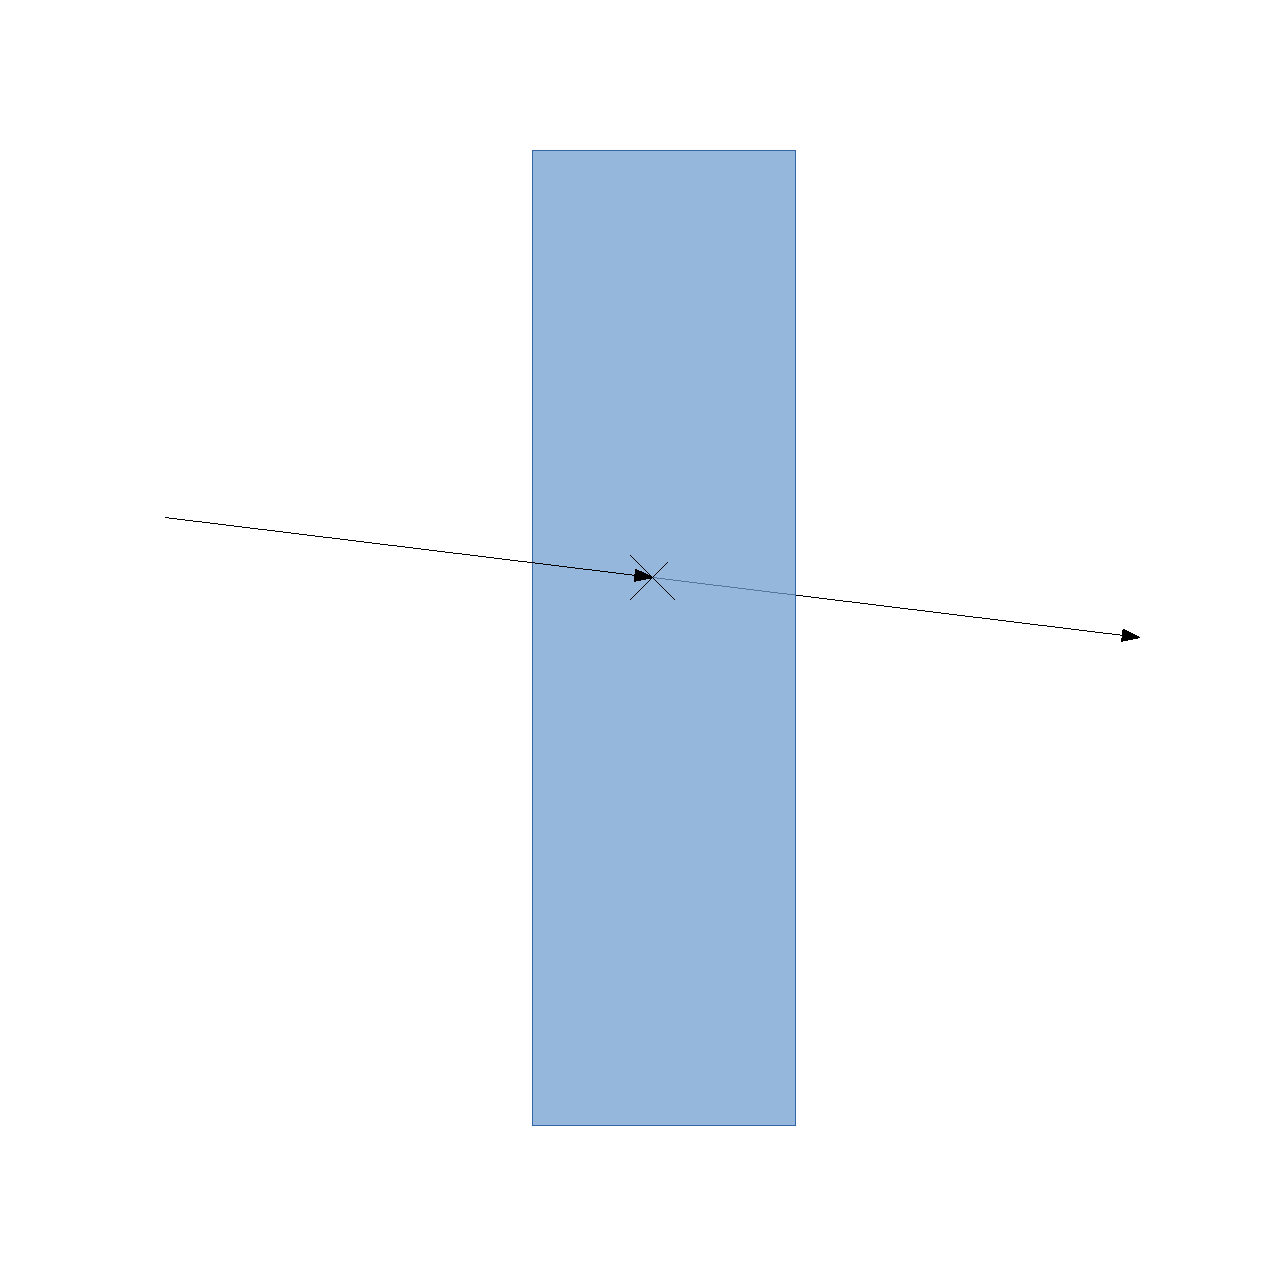
\includegraphics[angle=0,width=4in]{figures/bz.pdf}
      \caption{Graphical example of a decision tree.}
      \label{fig:dtree}
    \end{figure}
    
    A single tree can easily overfit a data set if it is at all complex, and
    its output is just a class label. Gradient-boosting addresses both of these
    issues by combining many weak classifiers into a strong one. Each weak
    classifier is built based on the error of the previous one. For a given
    training set, whenever a sample is classified incorrectly by a tree, that
    sample is given a higher importance when the next tree is being created.
    Mathematically, each tree is training on the gradient of the loss function.
    After all of the trees have been created, each tree is given a weight based
    on its ability to classify the training set, and the output of the
    gradient-boosted decision tree classifier is the probability that a sample
    is in a given class.
    
    The gradient-boosted decision tree software package we use is
    XGBoost~\cite{xgboost}. There are two types of classifiers we can use to
    separate protons from other tracks: binary and multiclass. Both classifiers
    are trained on all types of reconstructed tracks. A binary classifier
    classifies each track as either a proton or not a proton, and a multiclass
    classifier classifies a track as one of many types including a proton. We
    choose to use multiclass because the information about non-proton tracks is
    useful for event identification. The five classes that we train the
    decision trees to classify are protons (both BNB and cosmic), BNB muons,
    BNB pions, BNB electrons/photons, and all non-proton cosmics.
    
    The decision trees were trained to select protons in general. The target
    class contains all protons from BNB interactions, as well as cosmic
    protons. However, the choice of track features and most of the improvements
    that were made were done with the goal of a high efficiency for isolated
    protons and cosmic rejection.

  \subsubsection{Training}
    Describe the training sets. What samples were used, how many of everything,
    and all hyperparamter settings. Describe hyperparameter optimization. 
  \subsubsection{Performance}
    Show efficiency, accuracy, itemize backgrounds.
    Discuss reasons for different backgrounds.
  \subsubsection{Event selection}
    Need to select both NCE and CCQE events.
    Use particle ID plus reconstructed flashes.
    Exactly how we select NCE events 

%%%%%%%%%%%%%%%%%%%%%%%%%%%%%%%%%%%%%%%%%%%%%%%%%%%%%%%%%%%
% Efficiency and Background Estimation
%%%%%%%%%%%%%%%%%%%%%%%%%%%%%%%%%%%%%%%%%%%%%%%%%%%%%%%%%%%
\subsection{Efficiency and Background Estimation}\label{background}
  \subsubsection{Event selection efficiency}
    Efficiency due to TPC, PMT software trigger, reconstruction, proton ID,
    event selection, etc. This includes efficiency due to proton reinteracting
    in the nucleus and other nuclear effects.
  \subsubsection{Beam Induced Dirt Background}
    Discuss dirt neutrons, how they happen and estimated rates and energy
    distributions.  Show how well we can seperate or understand them. Show any
    sort of data-driven correction we did to dirt neutron background and how it
    affects our uncertainty. Talk about how well we can tag cryostat neutrons
    with the PMTs.
  \subsubsection{Beam Induced TPC Background}
    Talk about neutral-current elastic neutrons that are produced in the TPC
    and how their distributions differ from NCEp ones. Also include BNB
    backgounds (CCQE where muon wasn't reconstructed, NCpi0, etc.) Discuss how
    the optical signal would be different for each of these.
  \subsubsection{Cosmic Background}
    Discuss the difference between cosmic tracks and beam proton tracks. How do
    we separate them? What is the rate?

%%%%%%%%%%%%%%%%%%%%%%%%%%%%%%%%%%%%%%%%%%%%%%%%%%%%%%%%%%%
% Ratio of Cross Sections
%%%%%%%%%%%%%%%%%%%%%%%%%%%%%%%%%%%%%%%%%%%%%%%%%%%%%%%%%%%
\subsection{Ratio of NCEp to CCQEn Cross Sections}\label{ratios}
  Show how the ratio gets rid of a lot of measurement uncertainty like beam
  flux and efficiencies. Give exact equation that we will be using for
  analysis. Show how $\Delta s$ is still large at low $Q^2$.
  \subsubsection{Sources of Measurement Uncertainty}
    TPC efficiency: If ionization electrons actually reach the
    TPC and leave a signal.
    PMT trigger efficiency: Refer back to PMT trigger studies. Give uncertainty
    due to on signal.
    Reconstruction efficiency: Refer back. Give uncertainty on signal.
  \subsubsection{Quantifying Uncertainty on Ratio}\label{errorcalc}
    Calculate exact uncertainty and show it here.
  \subsubsection{}
    Nuclear effects and FSI. Discuss 

%%%%%%%%%%%%%%%%%%%%%%%%%%%%%%%%%%%%%%%%%%%%%%%%%%%%%%%%%%%
% Comparison to Simulation
%%%%%%%%%%%%%%%%%%%%%%%%%%%%%%%%%%%%%%%%%%%%%%%%%%%%%%%%%%%
\subsection{Comparison of data to simulation}
  \subsubsection{Reweighting}
  \subsubsection{Likelihood calculation}

%%%%%%%%%%%%%%%%%%%%%%%%%%%%%%%%%%%%%%%%%%%%%%%%%%%%%%%%%%%
% Joint Estimation
%%%%%%%%%%%%%%%%%%%%%%%%%%%%%%%%%%%%%%%%%%%%%%%%%%%%%%%%%%%
\subsection{Strange axial form factor parameter estimation}\label{deltas}
  Here is where we do the actual MCMC.
  \subsubsection{Bayesian inference}
    Walk through the Bayesian math. Start with wanting the probability of
    $\theta$ given the data and the model and get final equation. Then show how
    to combine with previous experiments. Should give detail for each factor in
    equation (prior, likelihood, posterior, evidence). Should especially give
    detail on how we choose priors. Maybe talk about model selection when
    talking about the evidence.
  \subsubsection{Markov Chain Monte Carlo}
    Go through detail on our implementation of MCMC. Discuss how Markov Chains
    work in general. Describe Metropolis, Gibbs, and our combination of both.
  \subsubsection{Results}
    Lots of plots! $\Delta s$!


%This is the end of analysis section

\newpage
%\section{SAMPLE TEXT WITH GRAPHICS} \label{graphics}
%This file illustrates how include in your thesis graphical
 %output.
%The next line produces an indented paragraph to start the document
 %unit.  The LaTeX defaults start most units without indentations.
\hspace{\parindent}
This is sample text with graphics.
\begin{figure}[h]
  \centering
  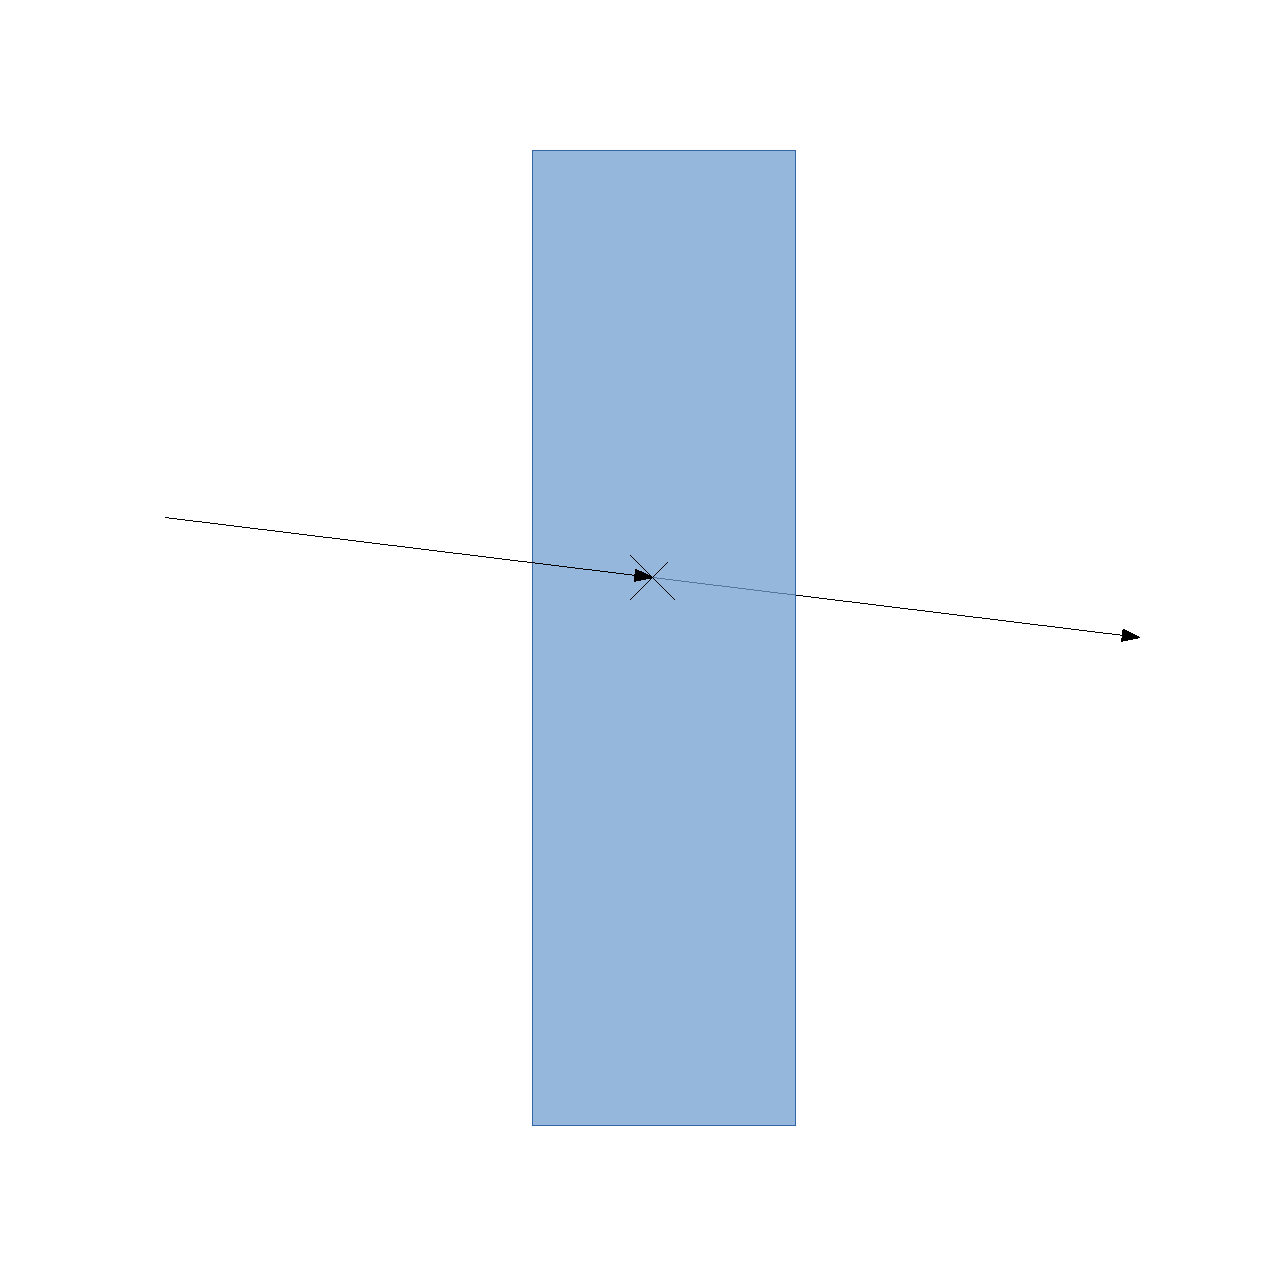
\includegraphics[angle=-90,width=4in]{figures/bz.pdf}
  \caption{This is an inserted EPS graphic}
  \label{fig:mygraph1}
\end{figure}
Sample ref of \ref{fig:mygraph1} 

\begin{figure}[t]
 \centering
  \includegraphics[angle=-90, width=4in]{figures/E734eta.pdf}  
    \caption{This is another inserted PDF graphic}
    \label{fig:mygraph2}
\end{figure}
%This is the end of the file graphics.tex


%\newpage
%The next four lines create a list of references for the 
 %paper from a .bbl file created by BibTeX from a .bib bibliographic
 %database file.  
 %The MathSciNet clipboard was used to prepare 
 %the .bib file.  See Lamport's book mentioned in the references for
 %basic information about BibTeX.  If you don't use BibTeX, you need
 %to create and format the list of references yourself.
\addcontentsline{toc}{section}{REFERENCES}
\setlength{\baselineskip}{\singlespace}
\bibliographystyle{plain}
\bibliography{main}
%These next three command lines create a list of references for the paper from
 %a biblio.tex file you create yourself.
%\addcontentsline{toc}{section}{REFERENCES}
%\setlength{\baselineskip}{\singlespace}
%%This file is a list of references prepared by hand.  If you are going 
 %to prepare your list of references by hand, you need to look
 %carefully at a journal and try  %to follow consistently the
 %journal's style.  
\begin{thebibliography}{99}

\bibitem{loday2} Fiedorowicz, Zbigniew  and Loday, Jean-Louis.
{\em Crossed Simplicial Groups and Their Associated Homology.}
Transactions of the American Mathematical Society, {\bf 36}(1991), p 57-87.

\bibitem{Higham}
Higham, Nicholas, J.  
{\em Handbook of writing for the mathematical sciences}, second edition.
Society for Industrial and Applied Mathematics, 1998.

\bibitem{Lamport} Lamport, Leslie.
{\em LaTeX:  A Document Preparation System}, Second Edition.
Addison-Wesley, (1994).

\bibitem{Lodaybook}Loday, Jean-Louis.
{\em Cyclic Homology.}
Springer Verlag, (1992).

\bibitem{L-Q} Loday, Jean-Louis and Quillen, Daniel.
{\em Cyclic Homology and the Lie Algebra Homology of Matrices.}
Comment. Math. Helv. {\bf 59}(1984), p 565-591.

\bibitem{Reckdahl}  Reckdahl, Keith.
{\em Using EPS Graphics in \LaTeX\ $2_{\varepsilon}$ Documents}.
Preprint, 1997.
 
\bibitem{Swanson}  Swanson, Ellen.
{\em Mathematics into type,} revised edition.
American Mathematical Society, 1979.

\end{thebibliography}
%This is the end of the file biblio.tex














%
\end{document}
